\section{Documentation}

L'application \appname~propose à ses utilisateurs la possibilité de découvrir les restaurants qui l'entourent sur son campus. Cette application est également destinée aux restaurateurs qui peuvent ainsi inscrire leur restaurant et donner des informations sur le menu du jour ou les offres promotionnelles ainsi que les évènements qu'ils organisent.

\todo{Réorganiser les descriptions avec les screenshots}

\begin{figure}[H]
    \label{fig-alarmes}
    \noindent\makebox[\textwidth]{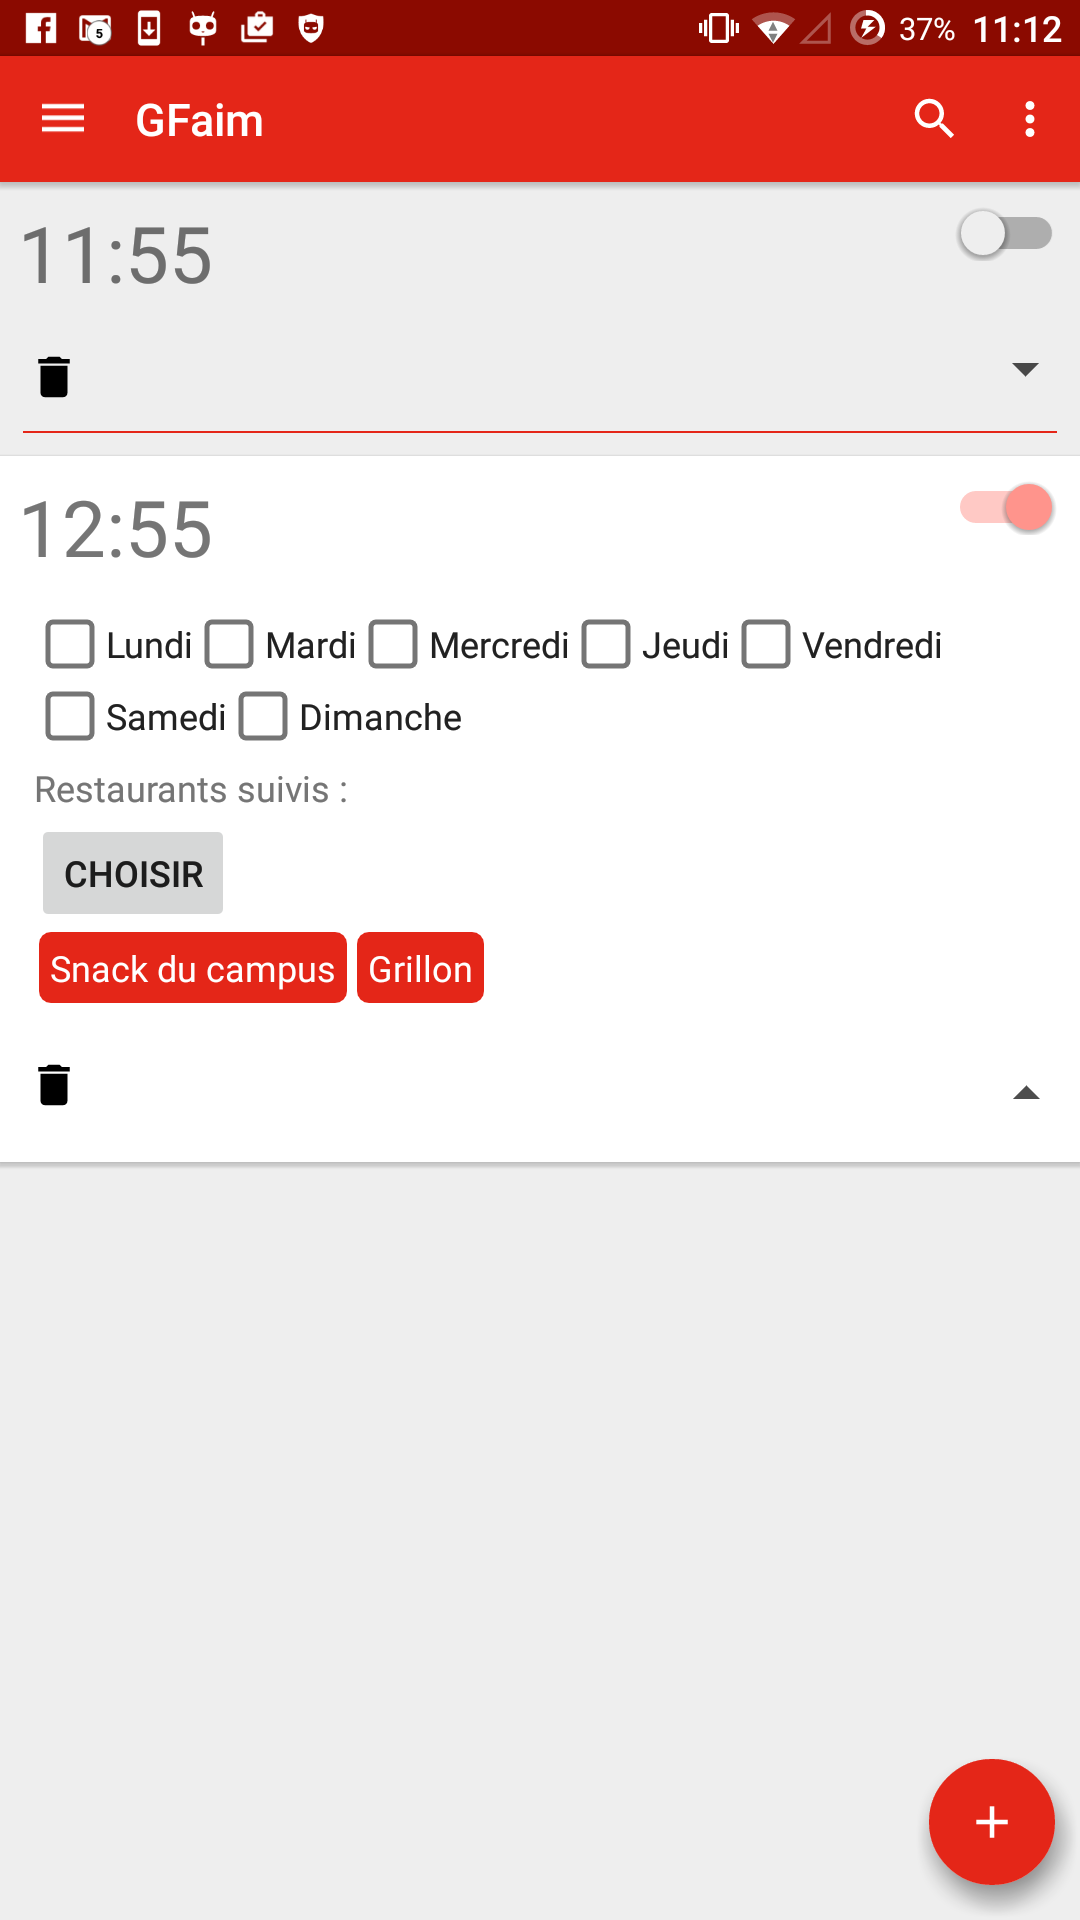
\includegraphics[width=8cm]{figures/screenshots/screenshot_alarme.png}}
    \caption{Capture d'écran des alarmes}
\end{figure}

\begin{figure}[H]
    \label{fig-carte}
    \noindent\makebox[\textwidth]{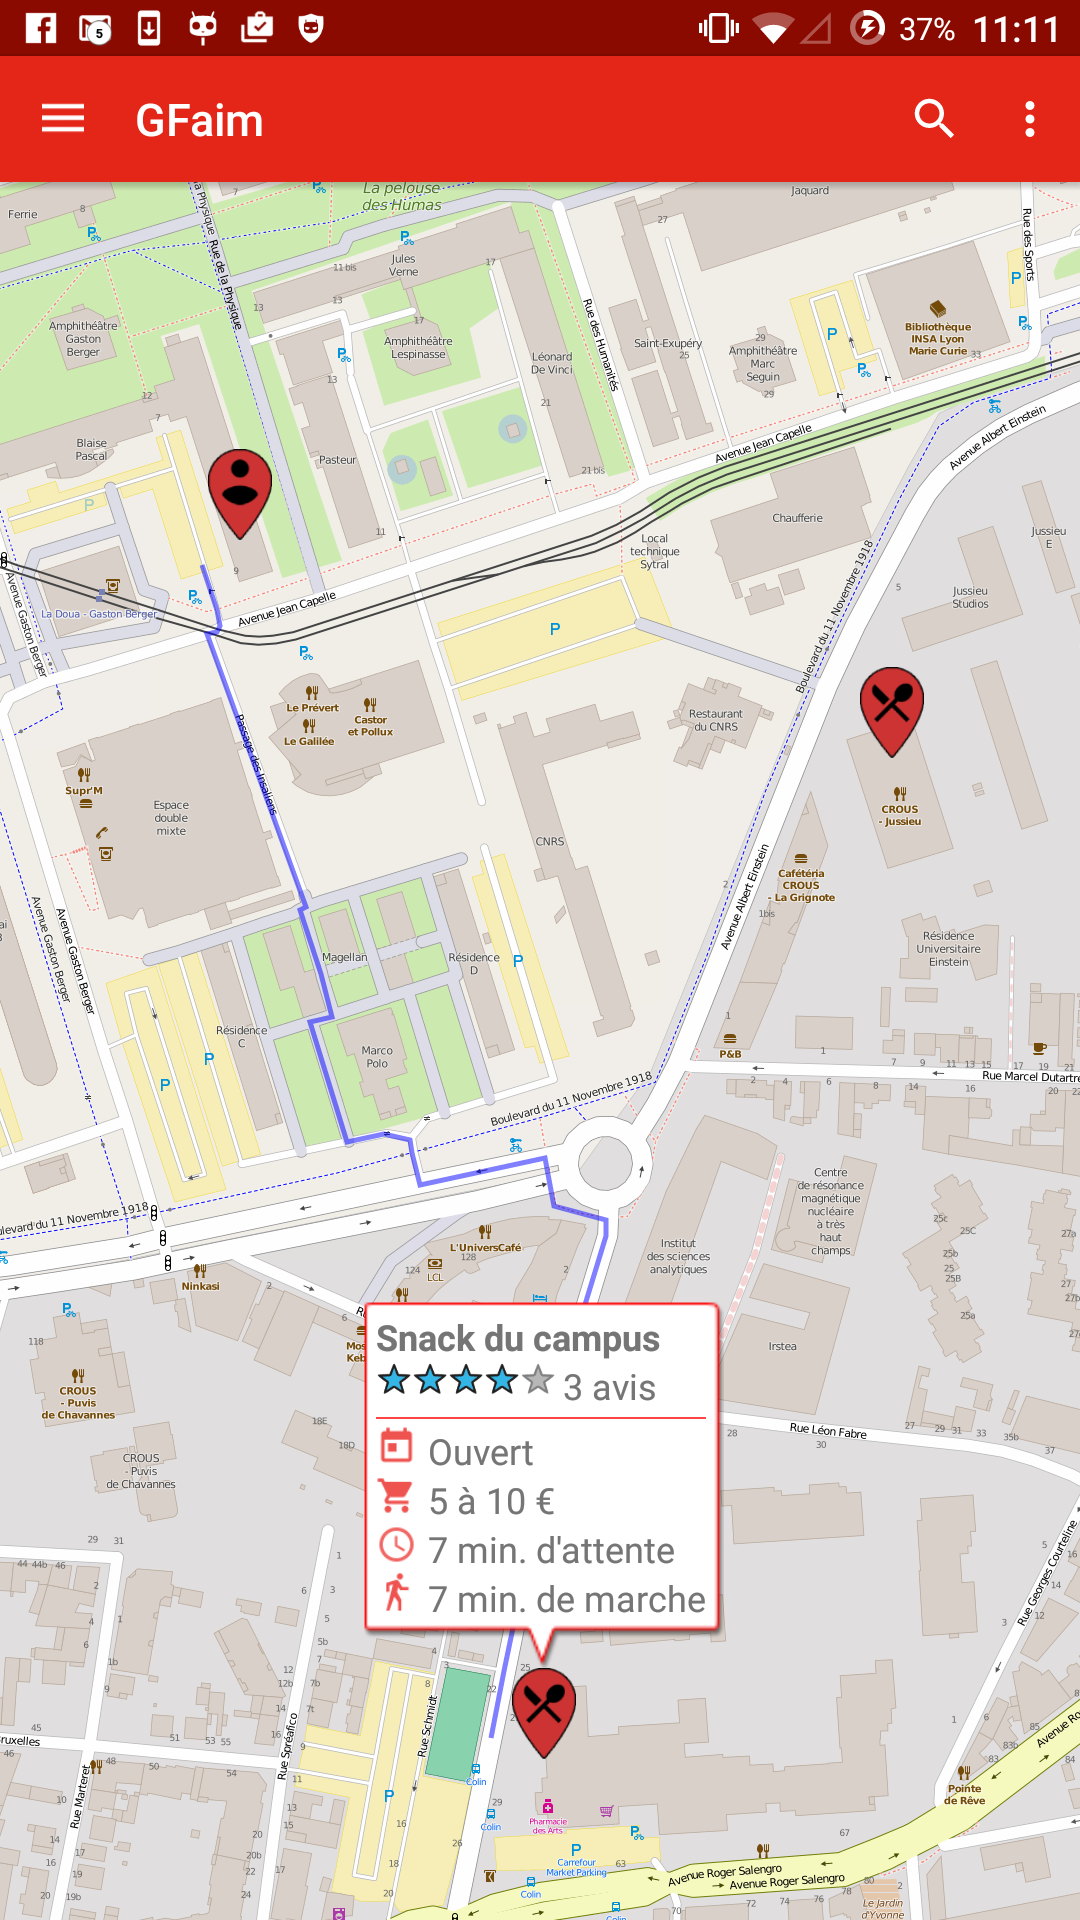
\includegraphics[width=8cm]{figures/screenshots/screenshot_carte.png}}
    \caption{Capture d'écran de la carte}
\end{figure}

\begin{figure}[H]
    \label{fig-contact}
    \noindent\makebox[\textwidth]{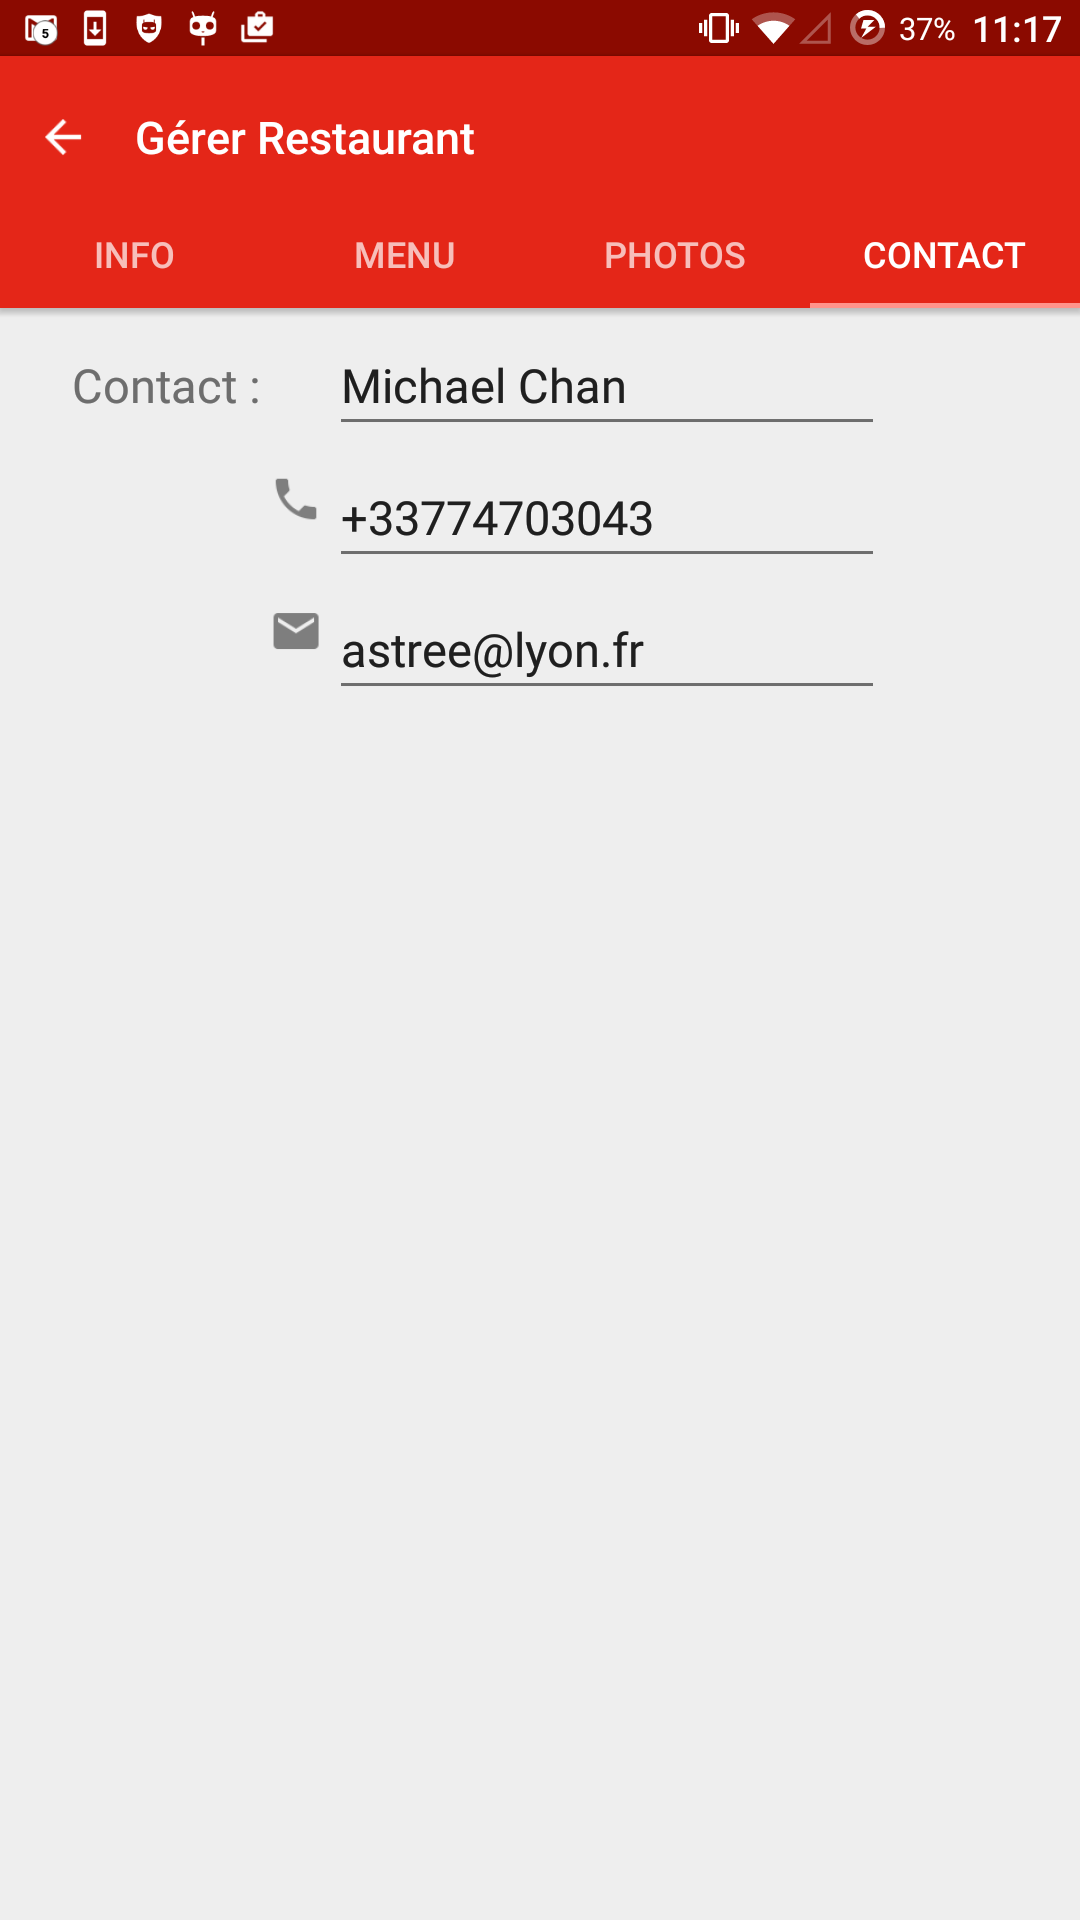
\includegraphics[width=8cm]{figures/screenshots/screenshot_contact.png}}
    \caption{Capture d'écran de la vue des contacts}
\end{figure}

\begin{figure}[H]
    \label{fig-detail-carte}
    \noindent\makebox[\textwidth]{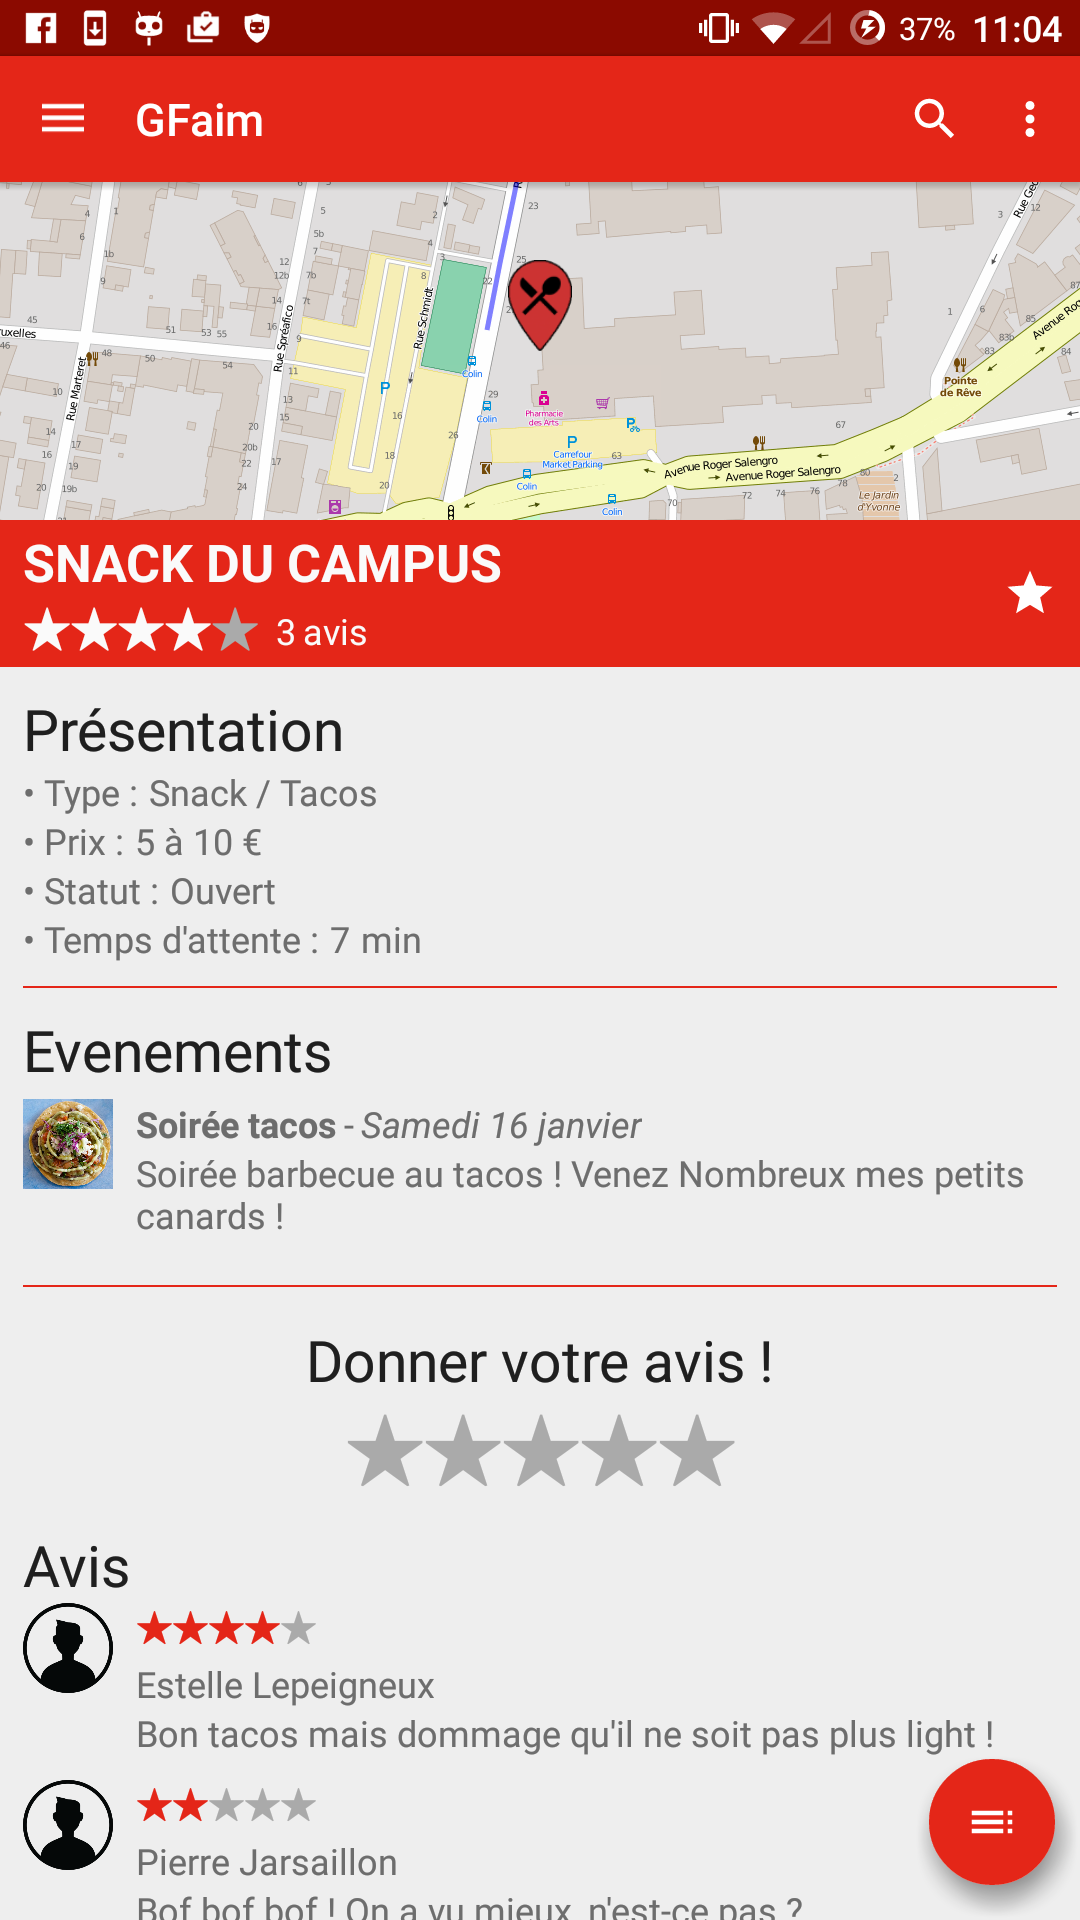
\includegraphics[width=8cm]{figures/screenshots/screenshot_detail_restaurant_carte.png}}
    \caption{Capture d'écran de la carte dans le detail du restaurant}
\end{figure}

\begin{figure}[H]
    \label{fig-detail-restaurant}
    \noindent\makebox[\textwidth]{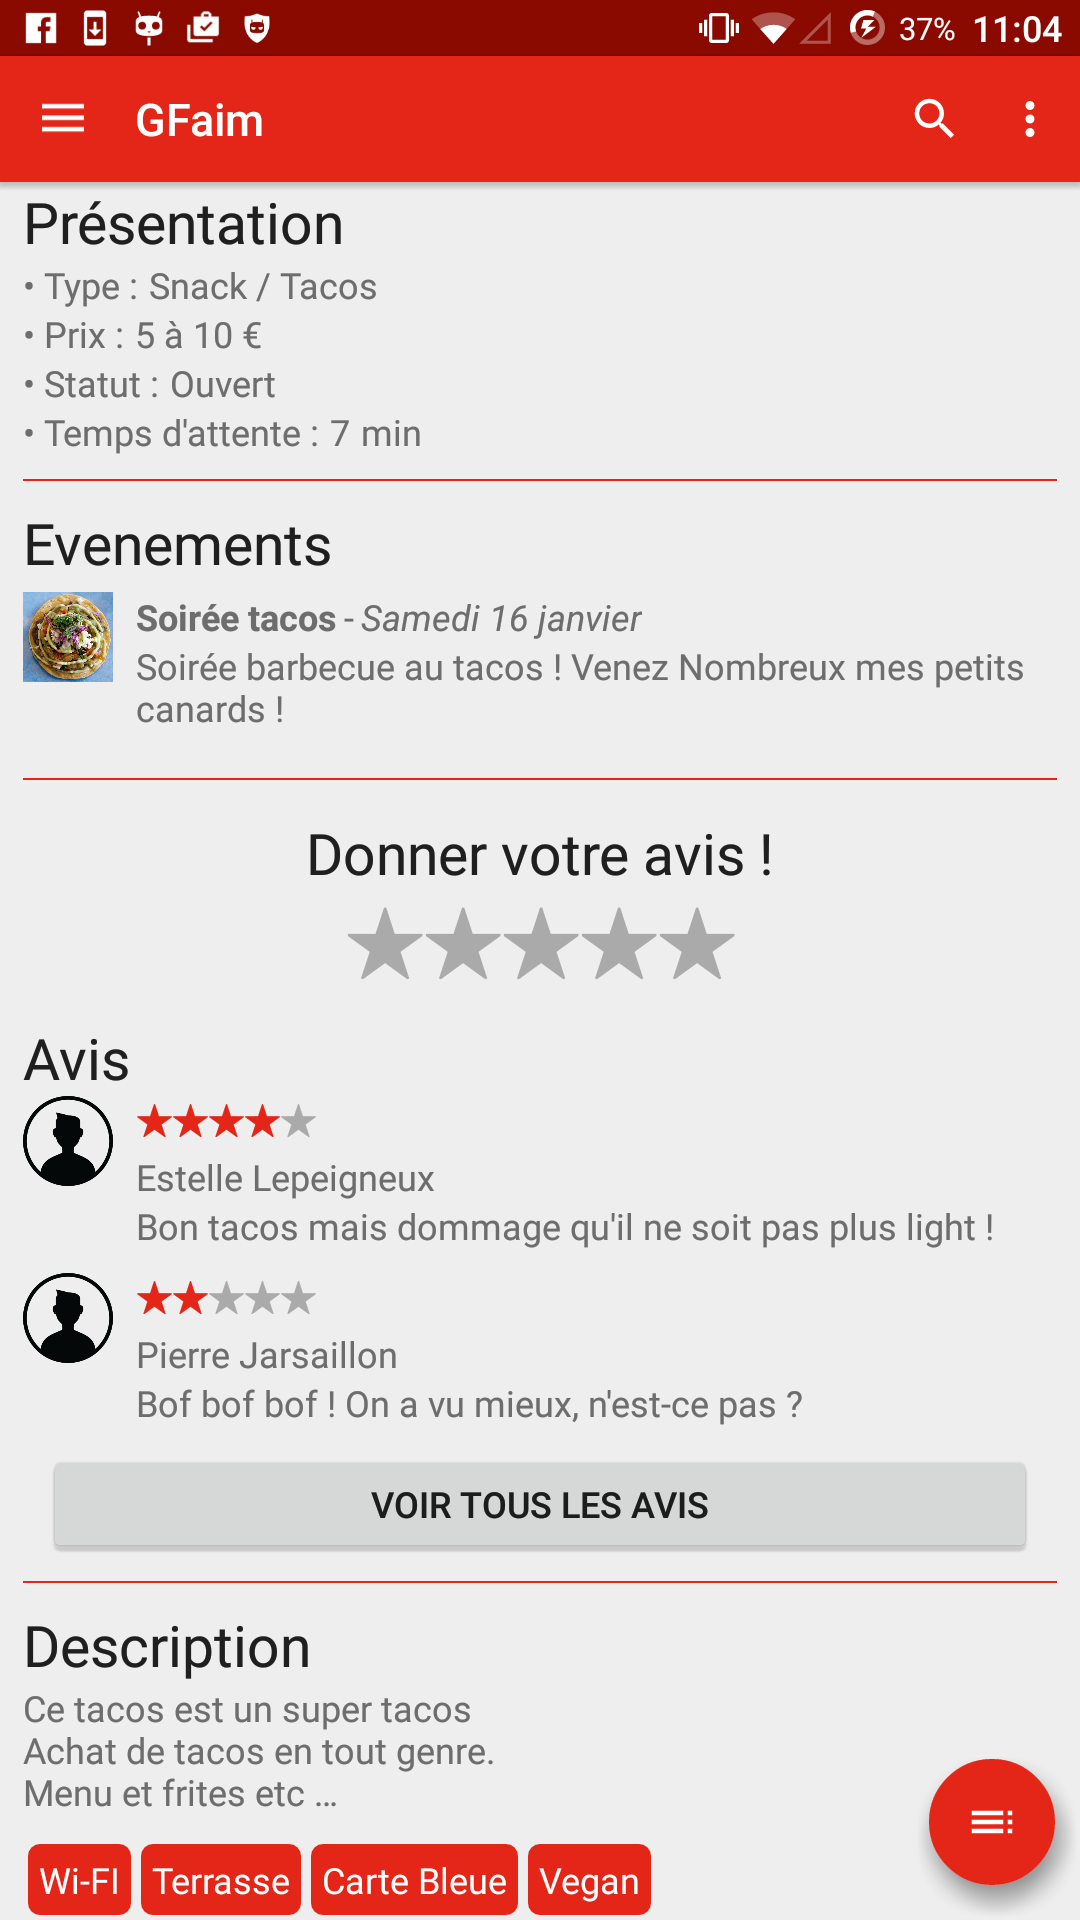
\includegraphics[width=8cm]{figures/screenshots/screenshot_detail_restaurant.png}}
    \caption{Capture d'écran du détail d'un restaurant}
\end{figure}

\begin{figure}[H]
    \label{fig-favoris}
    \noindent\makebox[\textwidth]{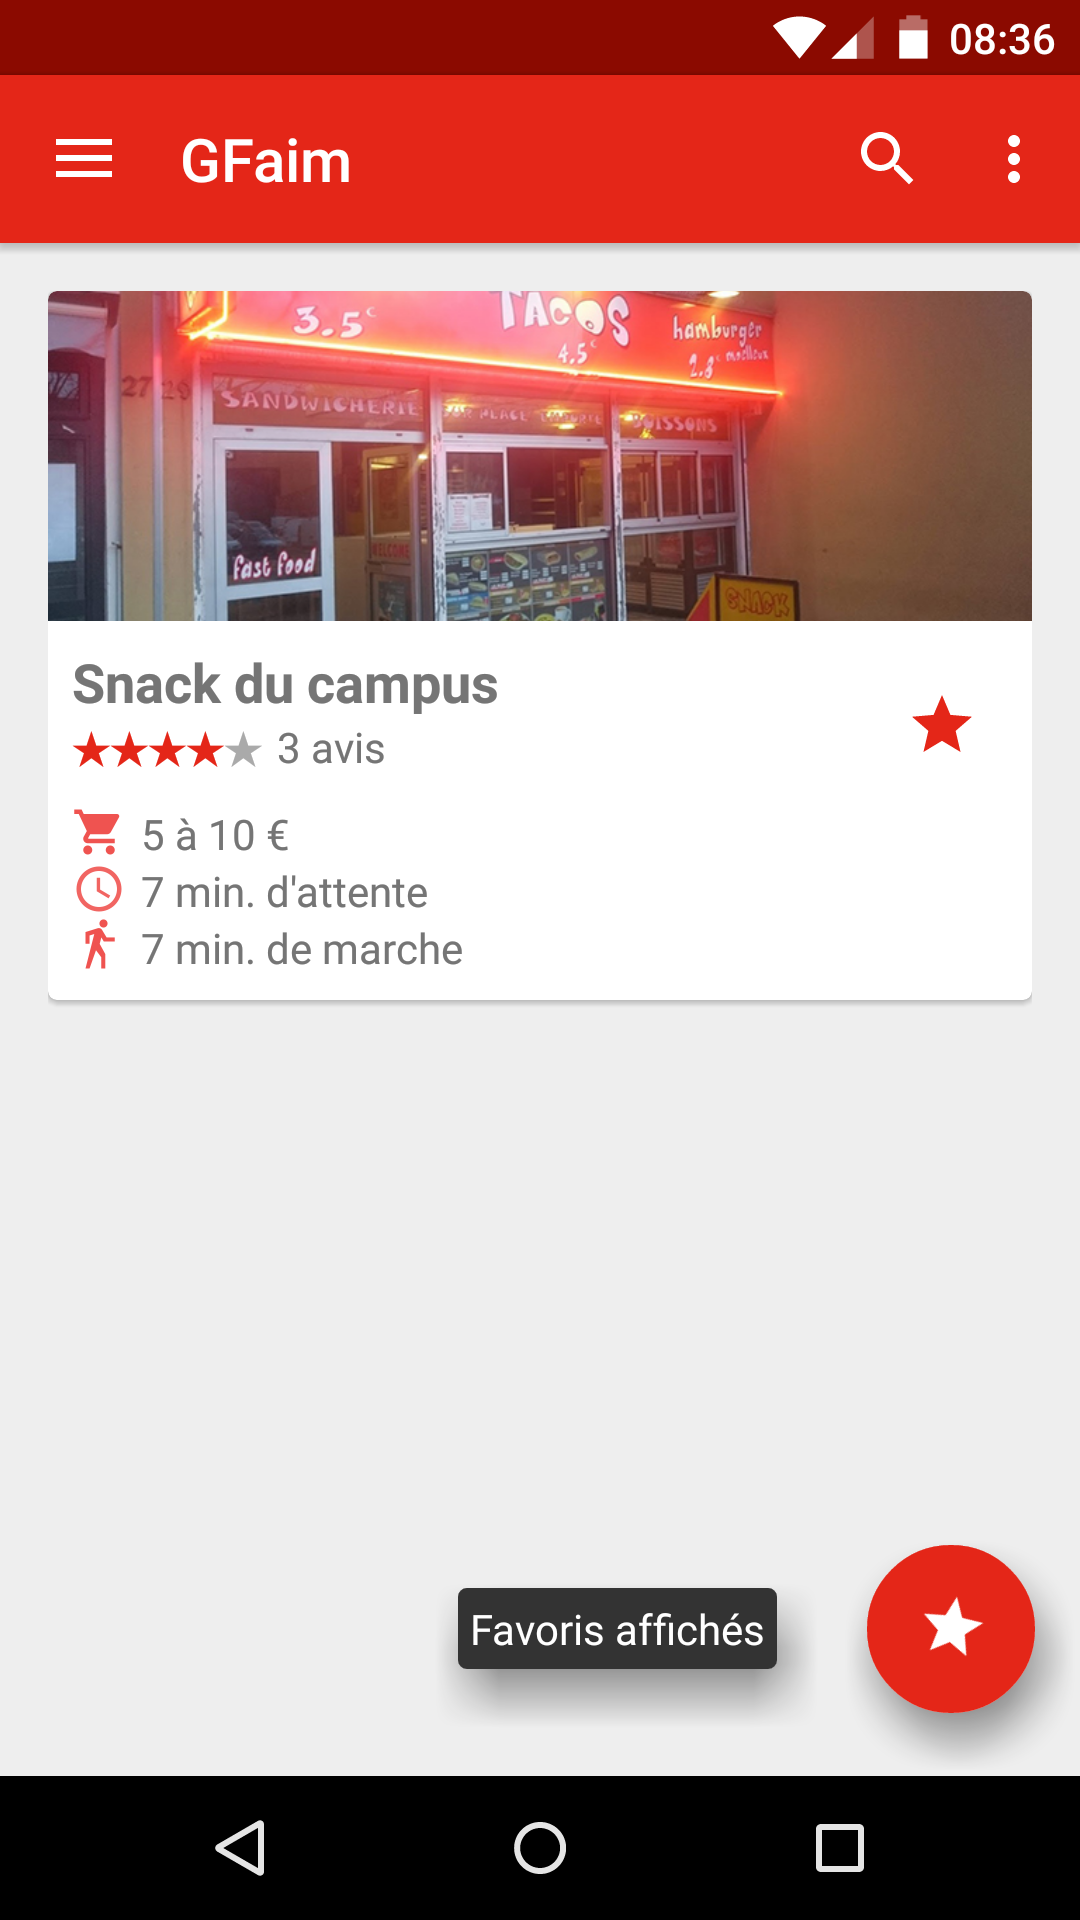
\includegraphics[width=8cm]{figures/screenshots/screenshot_favoris.png}}
    \caption{Capture d'écran des Restaurants Favoris}

\end{figure}

\begin{figure}[H]
    \label{fig-infos}
    \noindent\makebox[\textwidth]{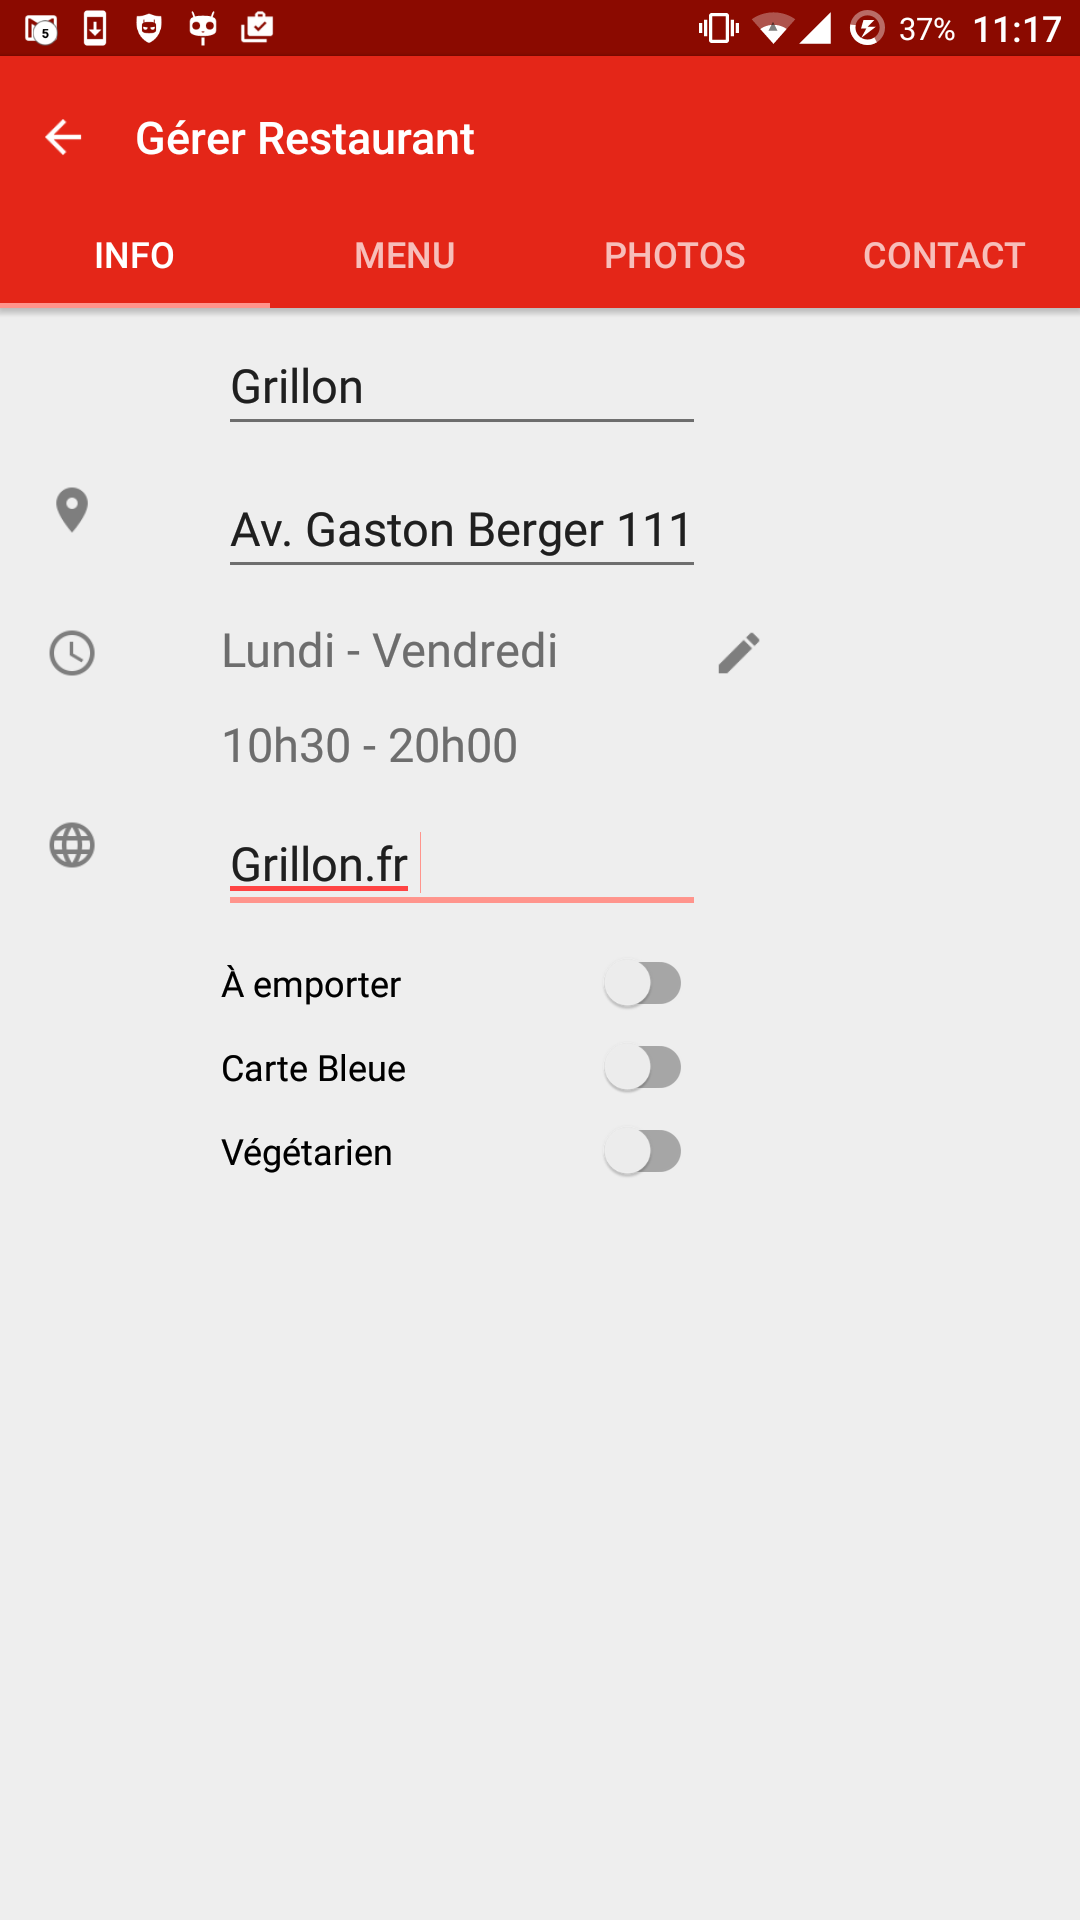
\includegraphics[width=8cm]{figures/screenshots/screenshot_infos.png}}
    \caption{Capture d'écran de la vue Informations}
\end{figure}

\begin{figure}[H]
    \label{fig-liste-restaurants}
    \noindent\makebox[\textwidth]{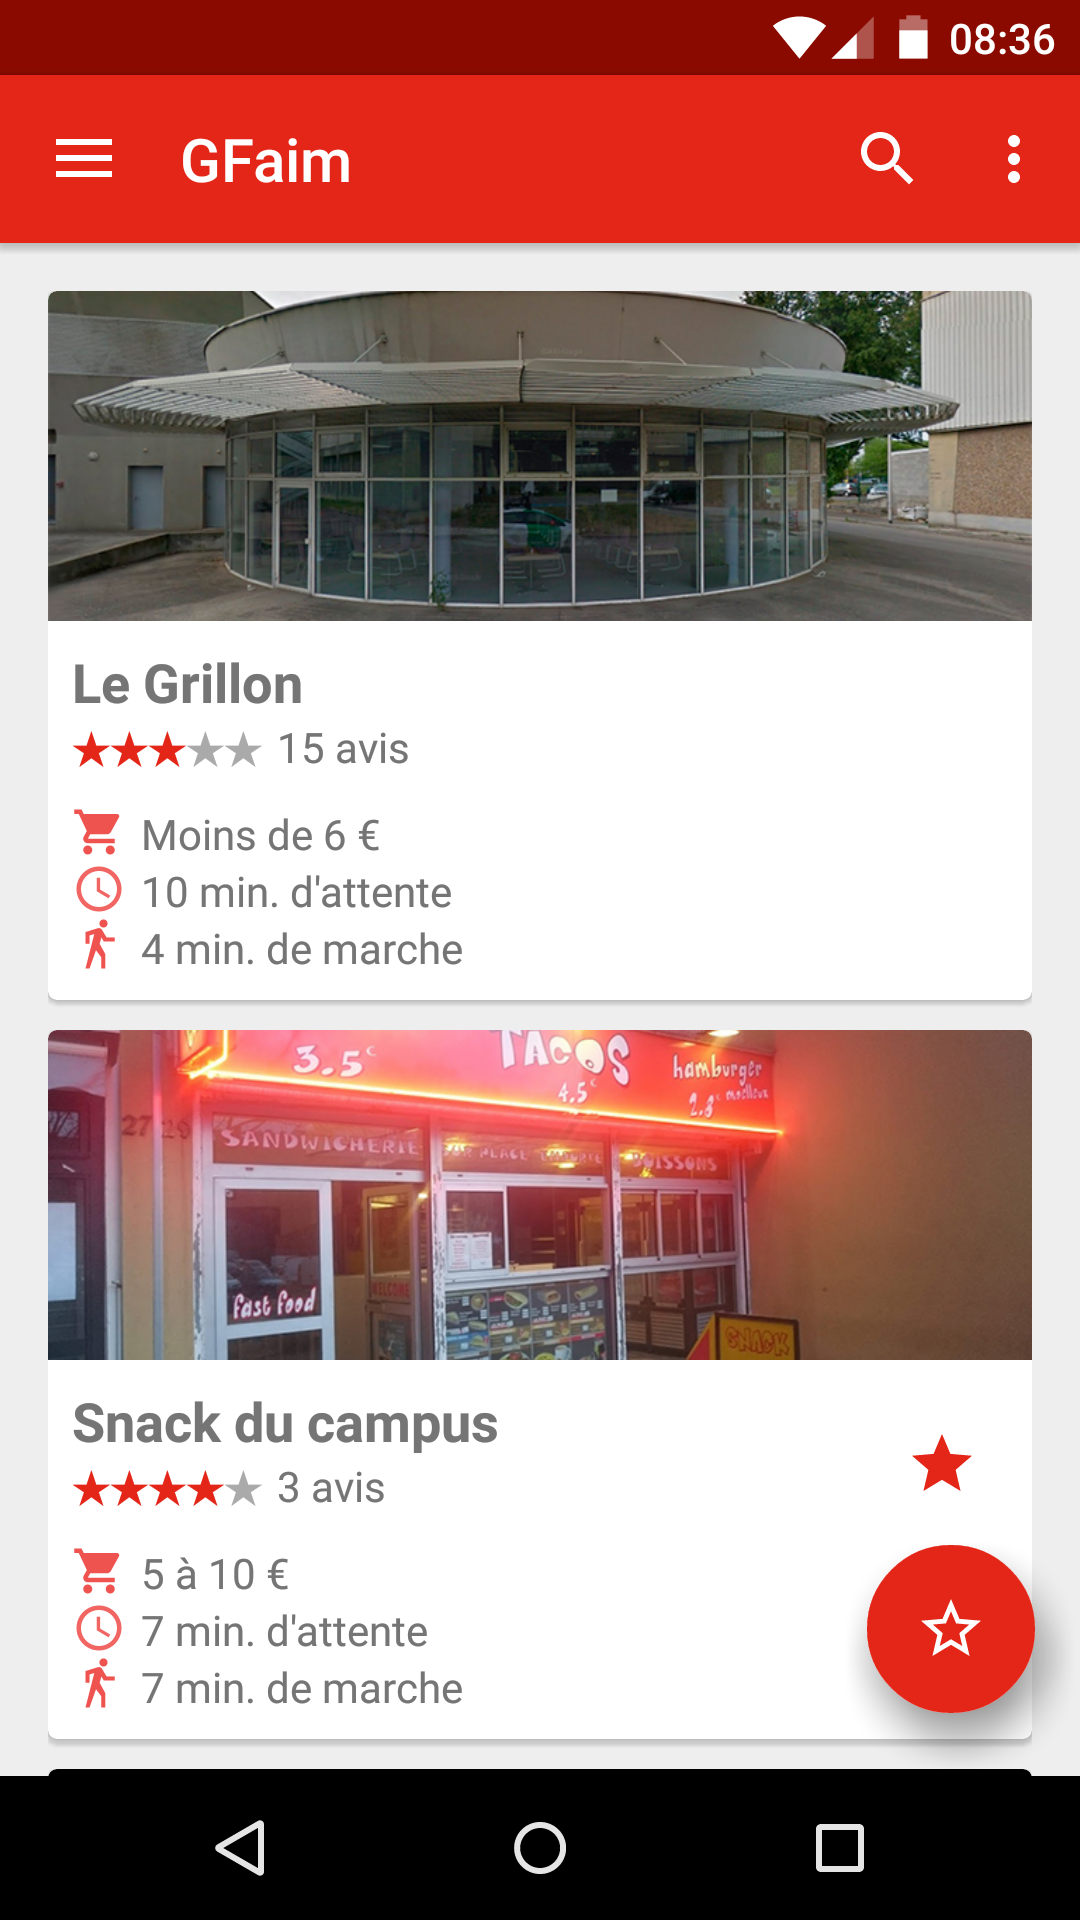
\includegraphics[width=8cm]{figures/screenshots/screenshot_liste_restaurant.png}}
    \caption{Capture d'écran de la Liste des Restaurants}
\end{figure}

\begin{figure}[H]
    \label{fig-login}
    \noindent\makebox[\textwidth]{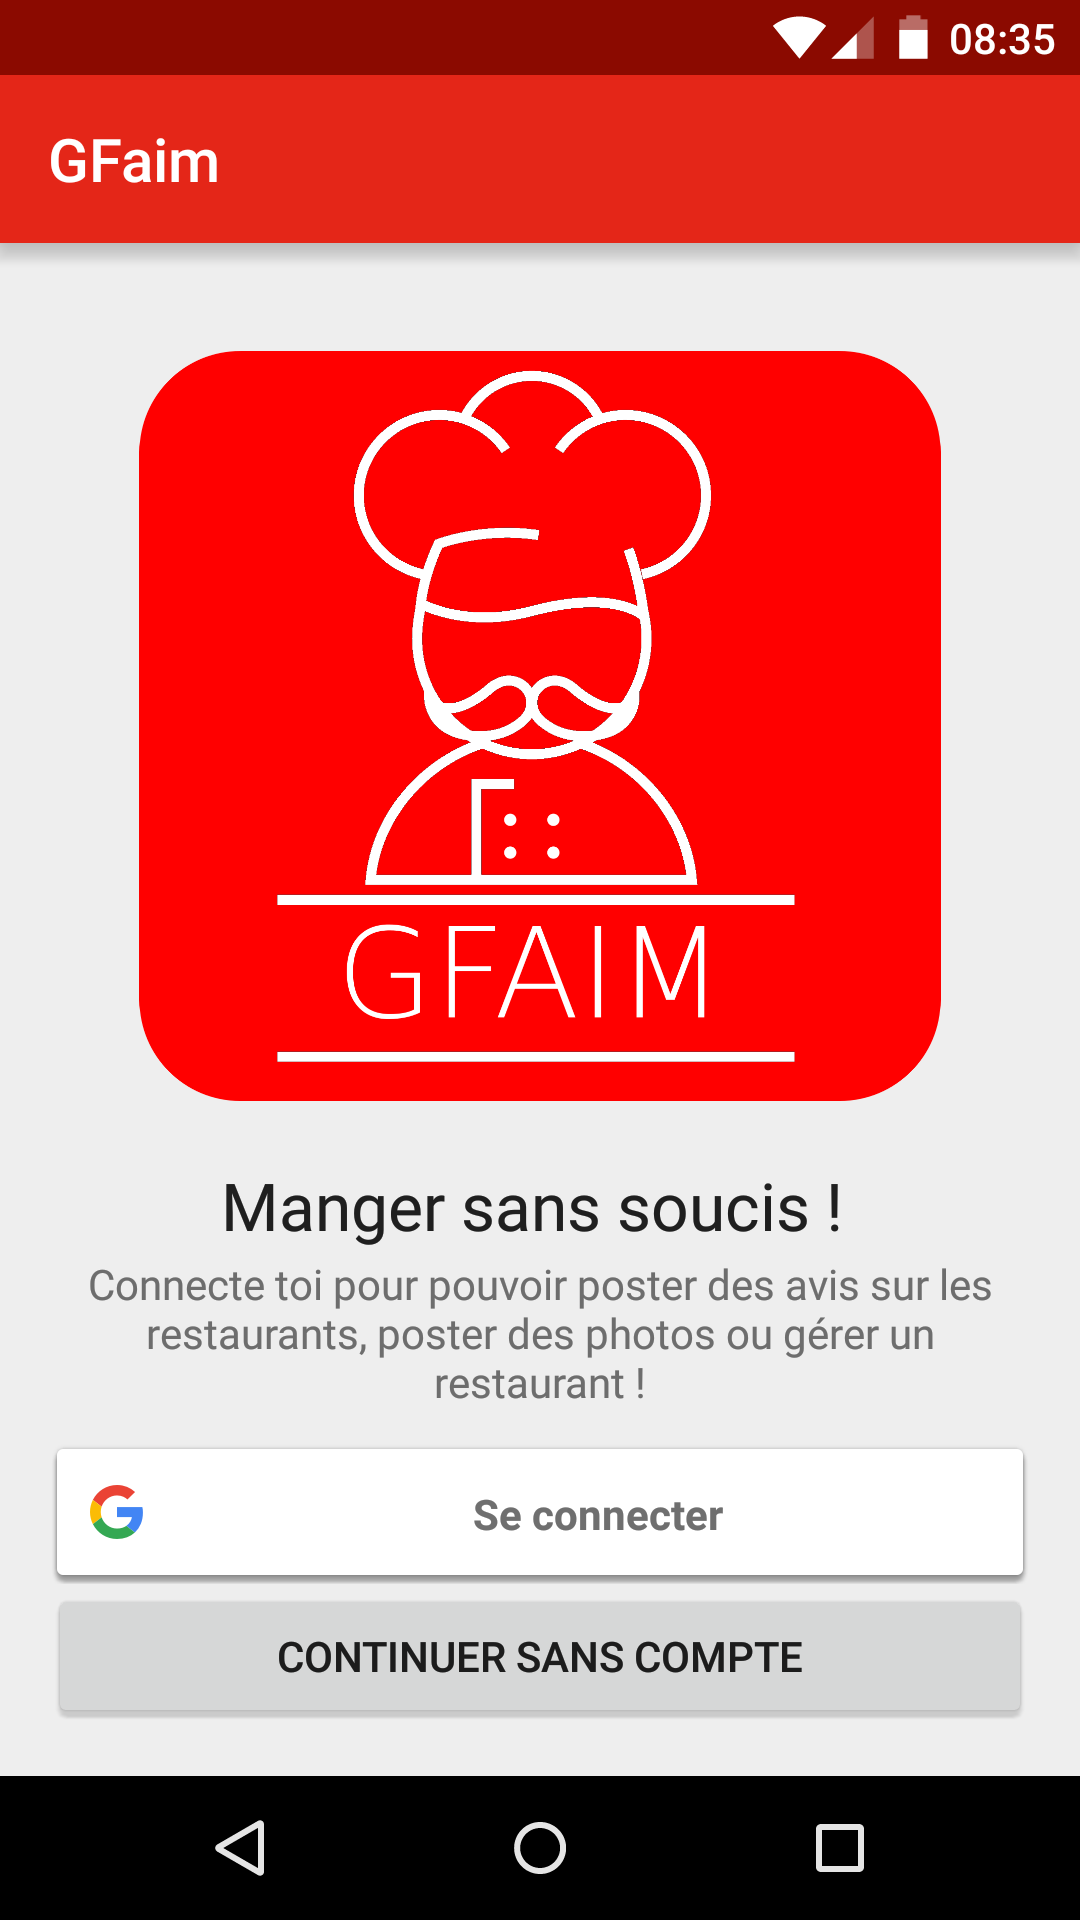
\includegraphics[width=8cm]{figures/screenshots/screenshot_login.png}}
    \caption{Capture d'écran de l'écran de connexion}
\end{figure}

\begin{figure}[H]
    \label{fig-menu-bulle}
    \noindent\makebox[\textwidth]{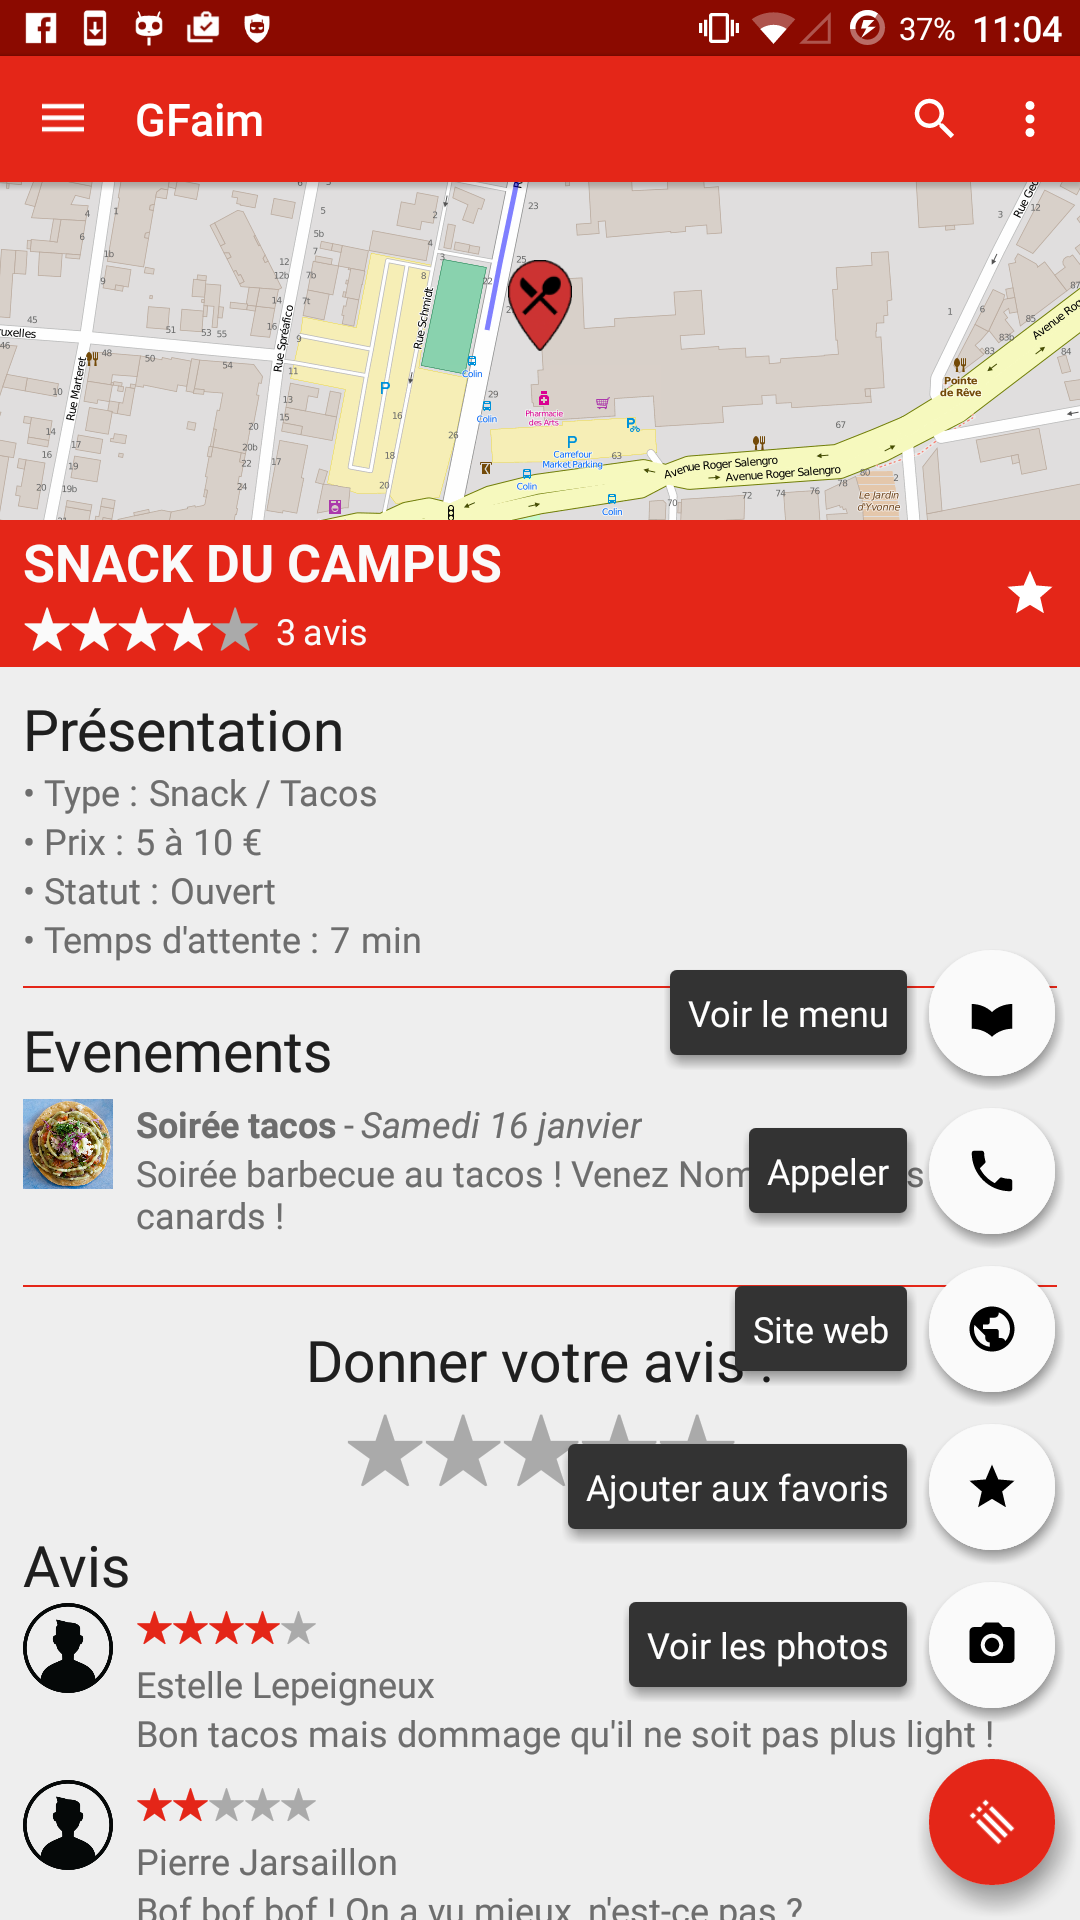
\includegraphics[width=8cm]{figures/screenshots/screenshot_menu_bulle.png}}
    \caption{Capture d'écran du menu bulle}
\end{figure}

\begin{figure}[H]
    \label{fig-menu-lateral}
    \noindent\makebox[\textwidth]{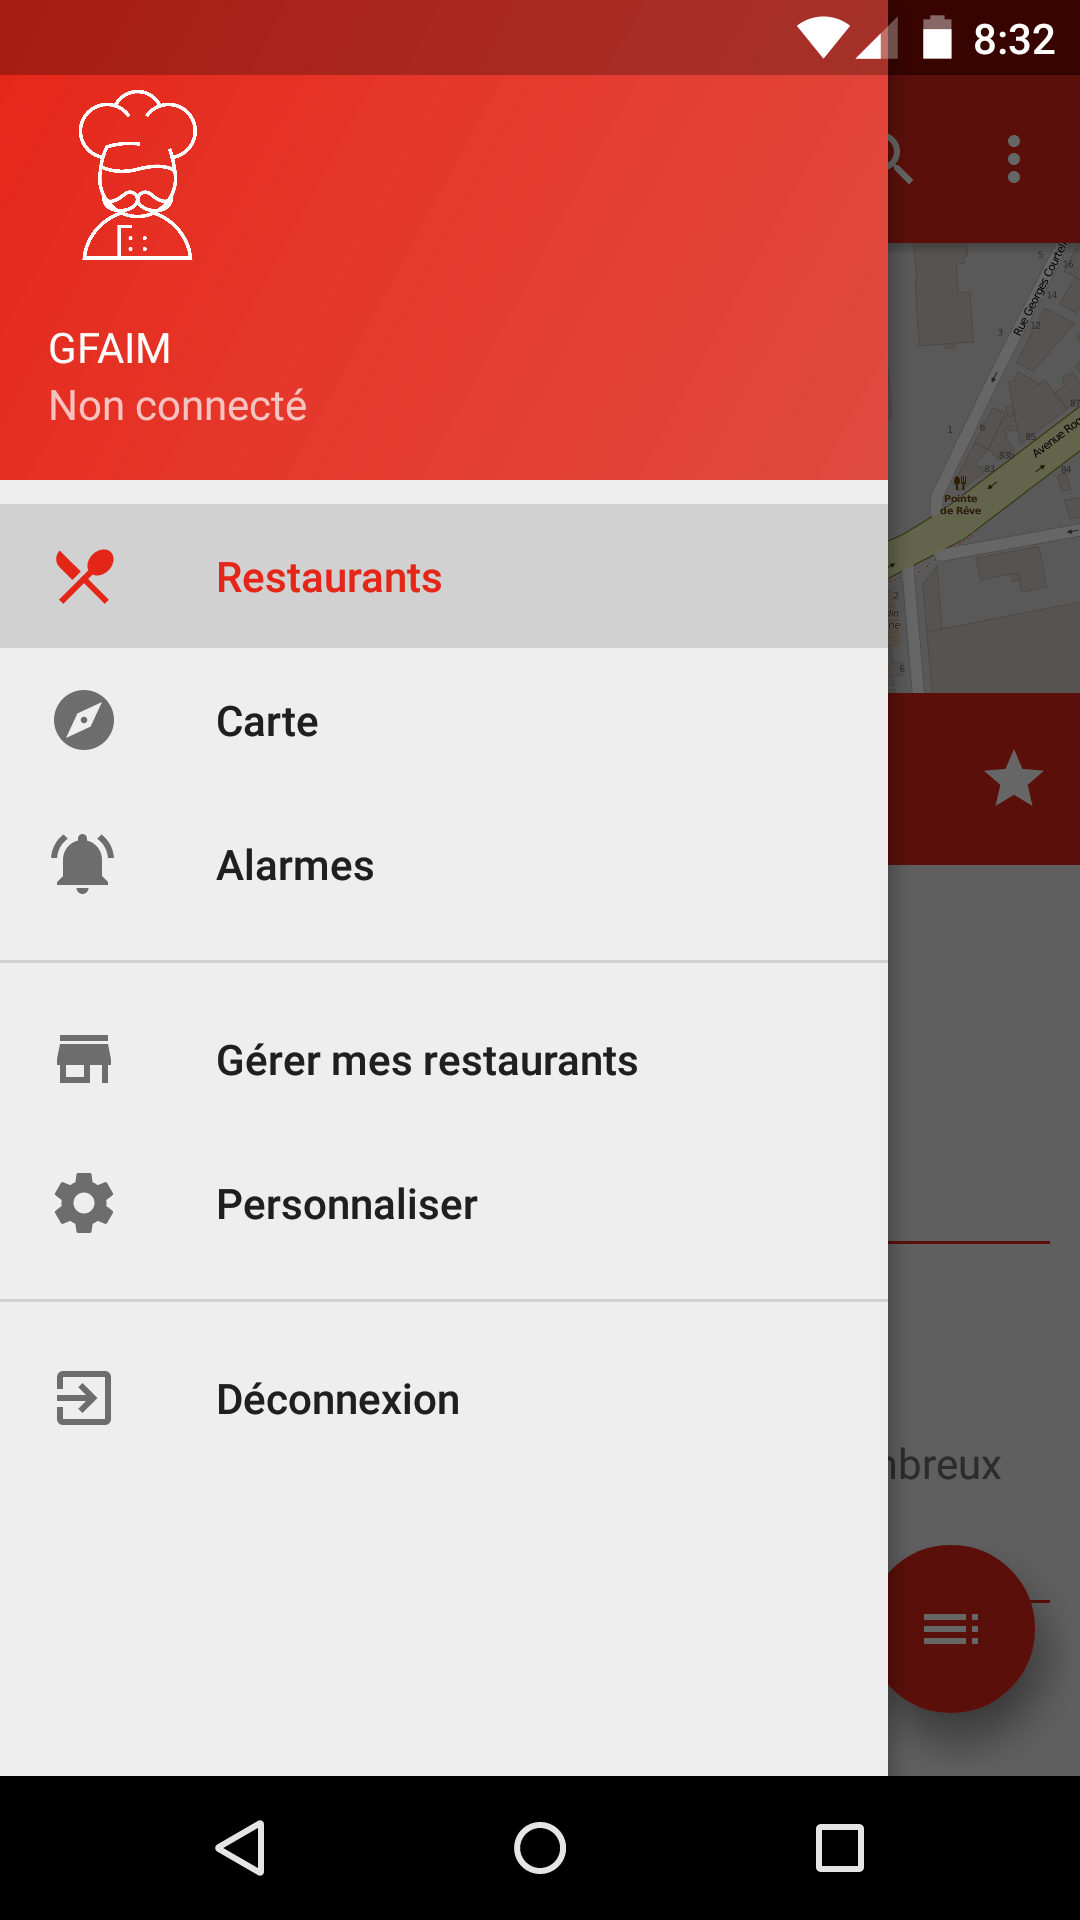
\includegraphics[width=8cm]{figures/screenshots/screenshot_menu_lateral.png}}
    \caption{Capture d'écran du menu volet à gauche}
\end{figure}

\begin{figure}[H]
    \label{fig-menu}
    \noindent\makebox[\textwidth]{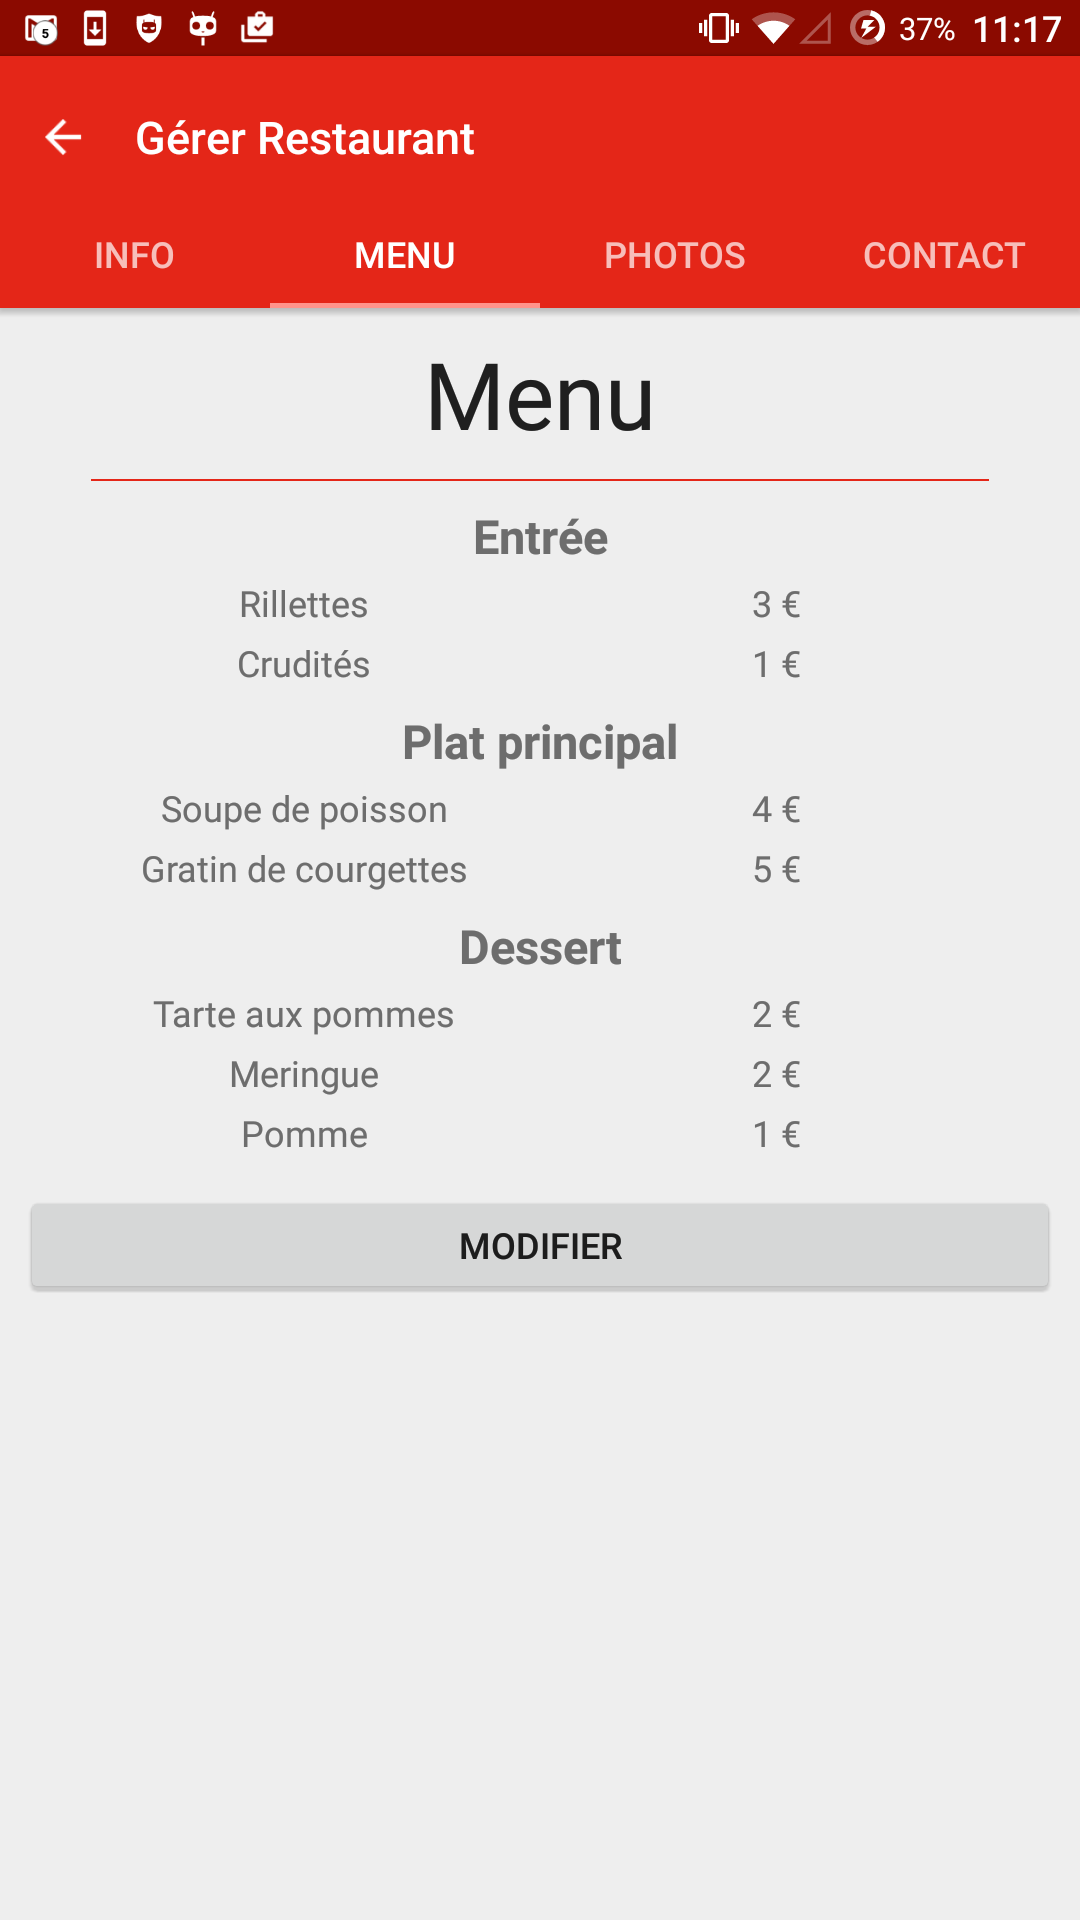
\includegraphics[width=8cm]{figures/screenshots/screenshot_menu.png}}
    \caption{Capture d'écran présentant le menu}
\end{figure}

\begin{figure}[H]
    \label{fig-menu-popup}
    \noindent\makebox[\textwidth]{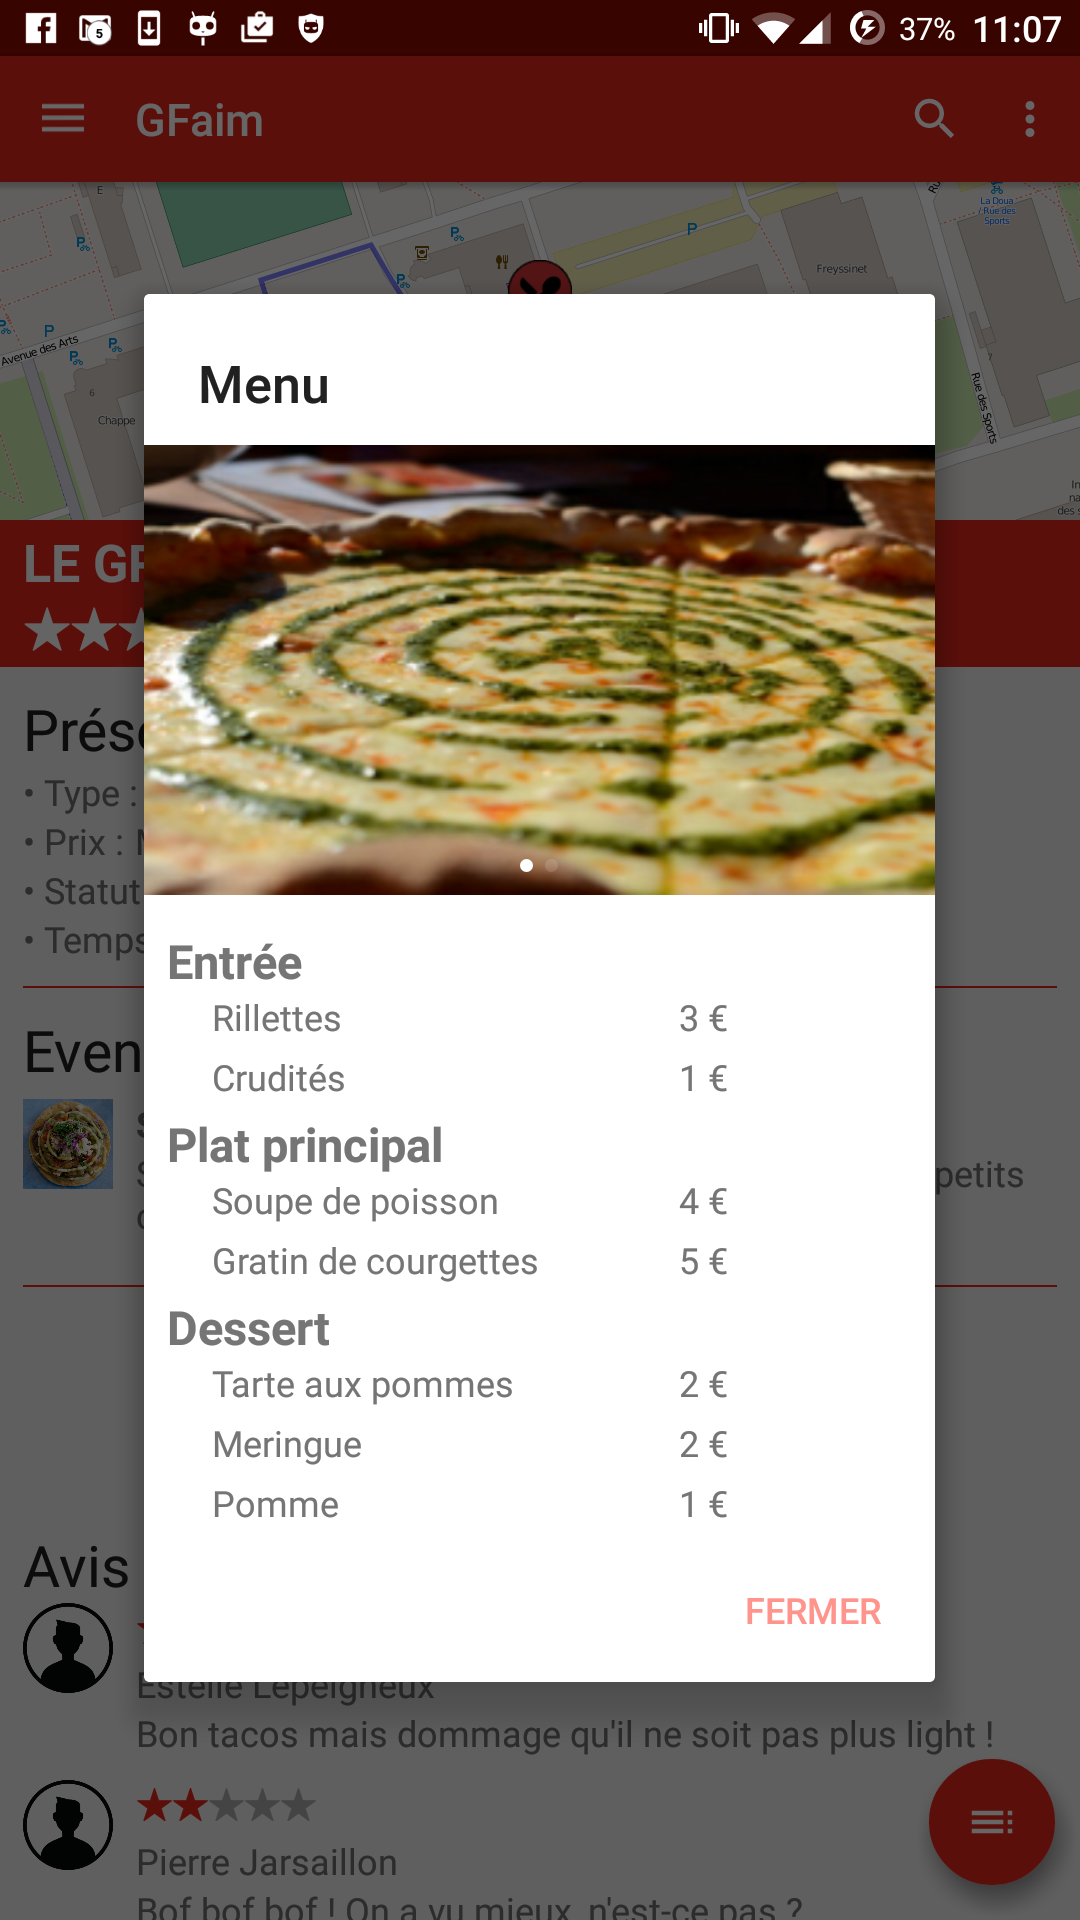
\includegraphics[width=8cm]{figures/screenshots/screenshot_menu_popup.png}}
    \caption{Capture d'écran du popup présentant le menu}
\end{figure}

\begin{figure}[H]
    \label{fig-mes-restaurants}
    \noindent\makebox[\textwidth]{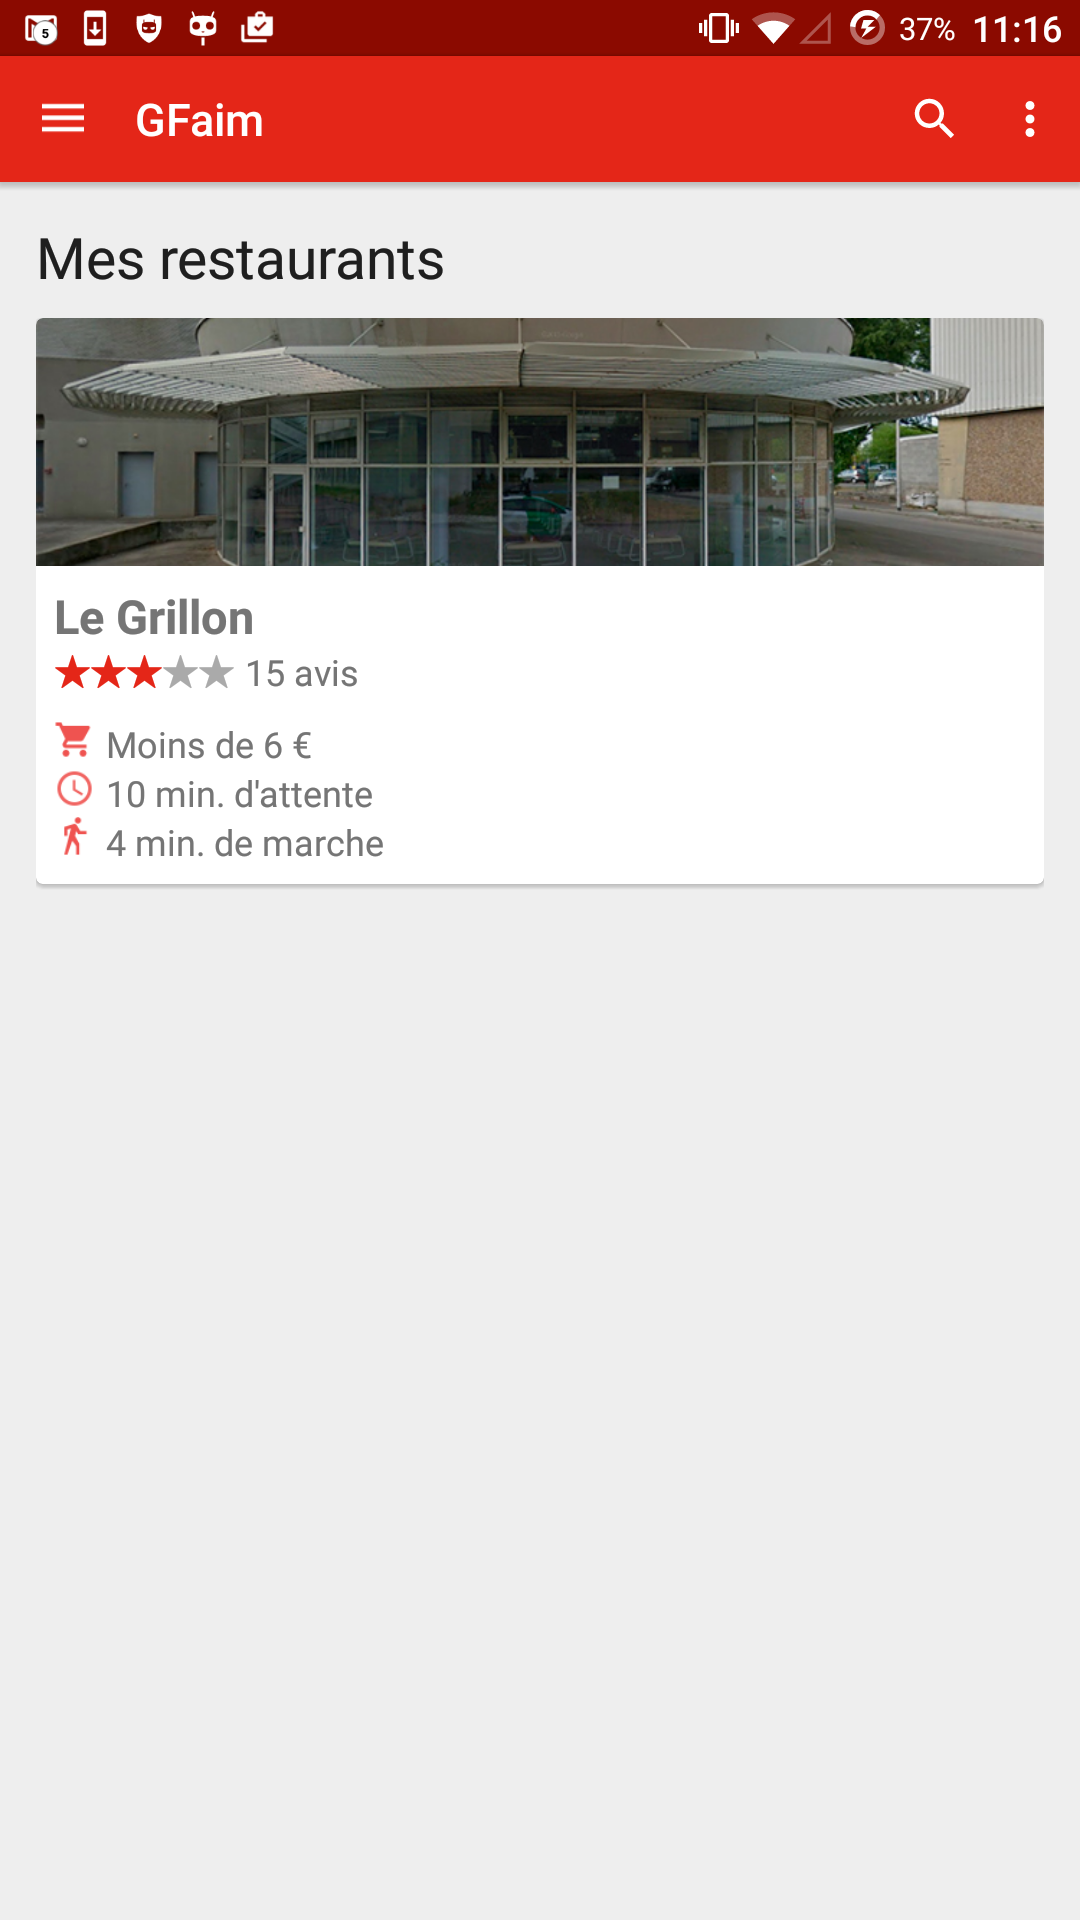
\includegraphics[width=8cm]{figures/screenshots/screenshot_mes_restaurants.png}}
    \caption{Capture d'écran de la liste Mes Restaurants}
\end{figure}

\begin{figure}[H]
    \label{fig-photos}
    \noindent\makebox[\textwidth]{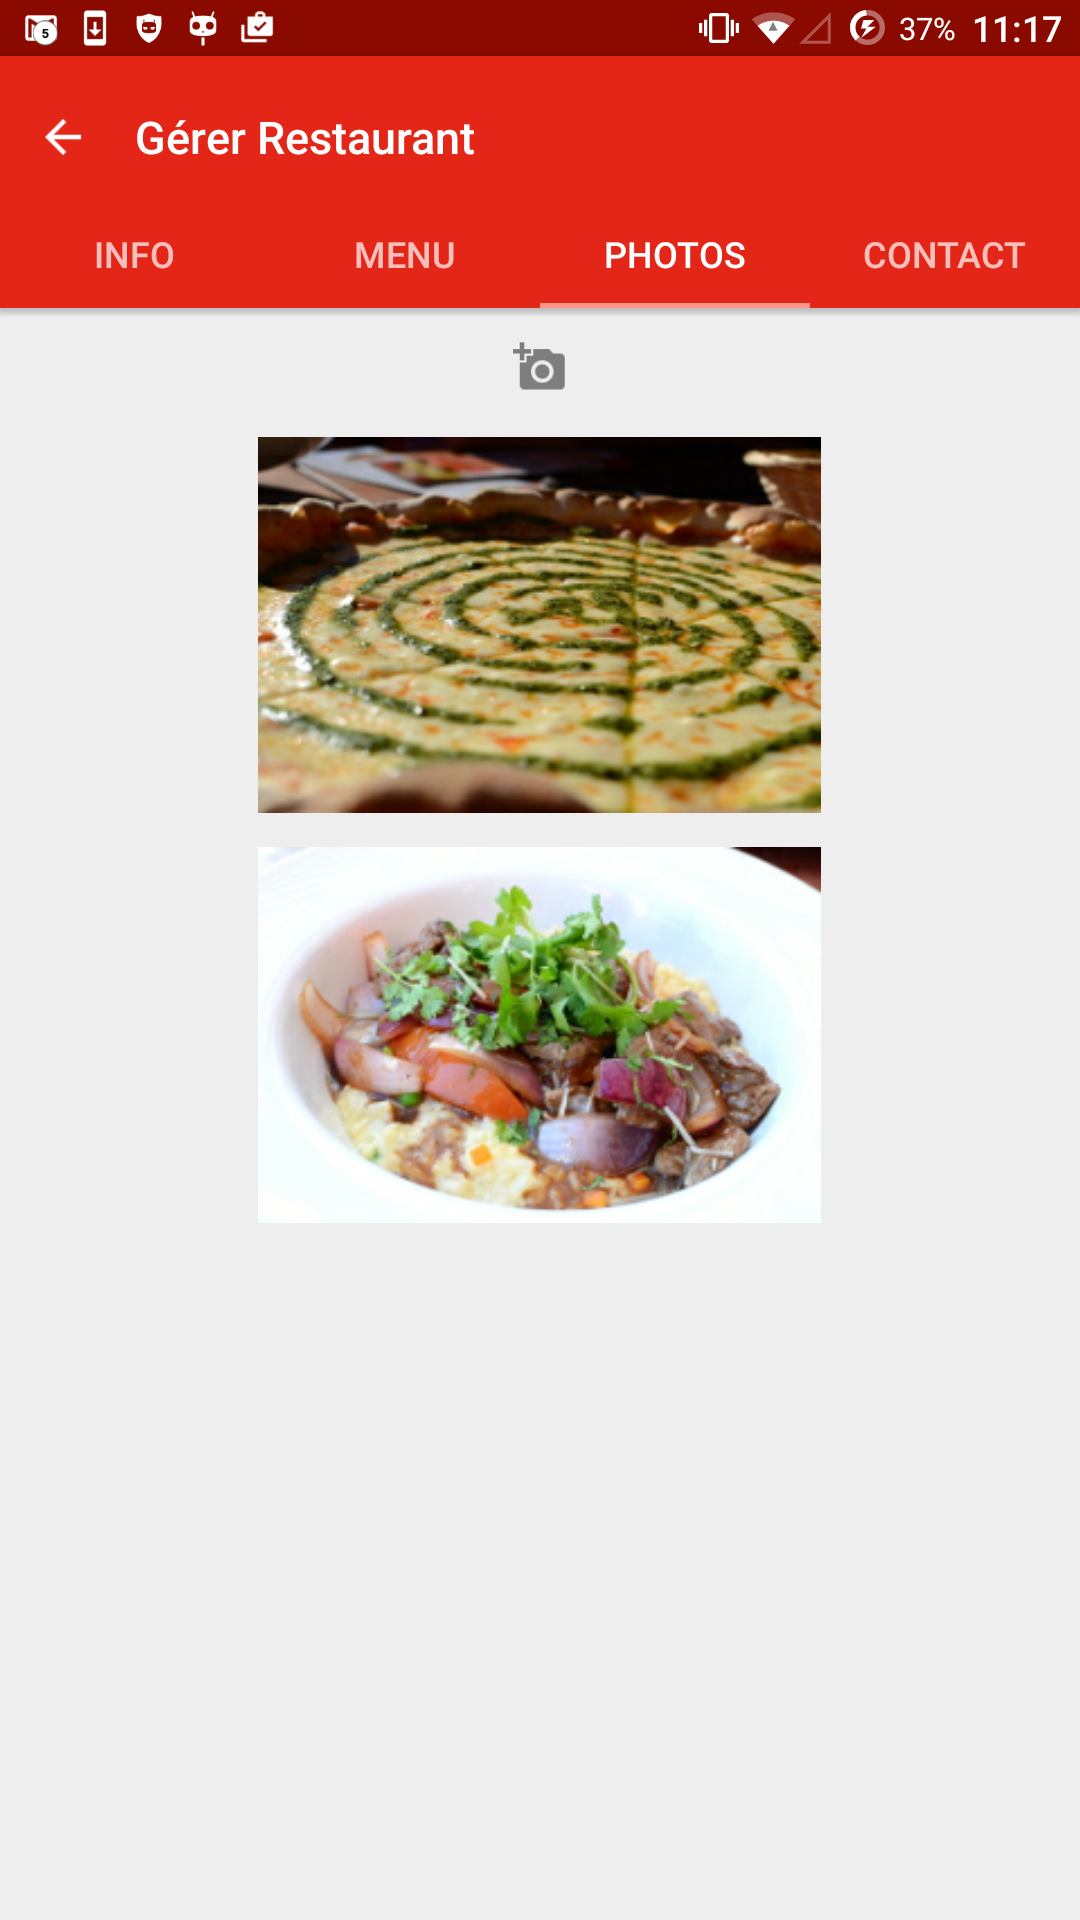
\includegraphics[width=8cm]{figures/screenshots/screenshot_photos.png}}
    \caption{Capture d'écran de la vue photos}
\end{figure}

\begin{figure}[H]
    \label{fig-preferences}
    \noindent\makebox[\textwidth]{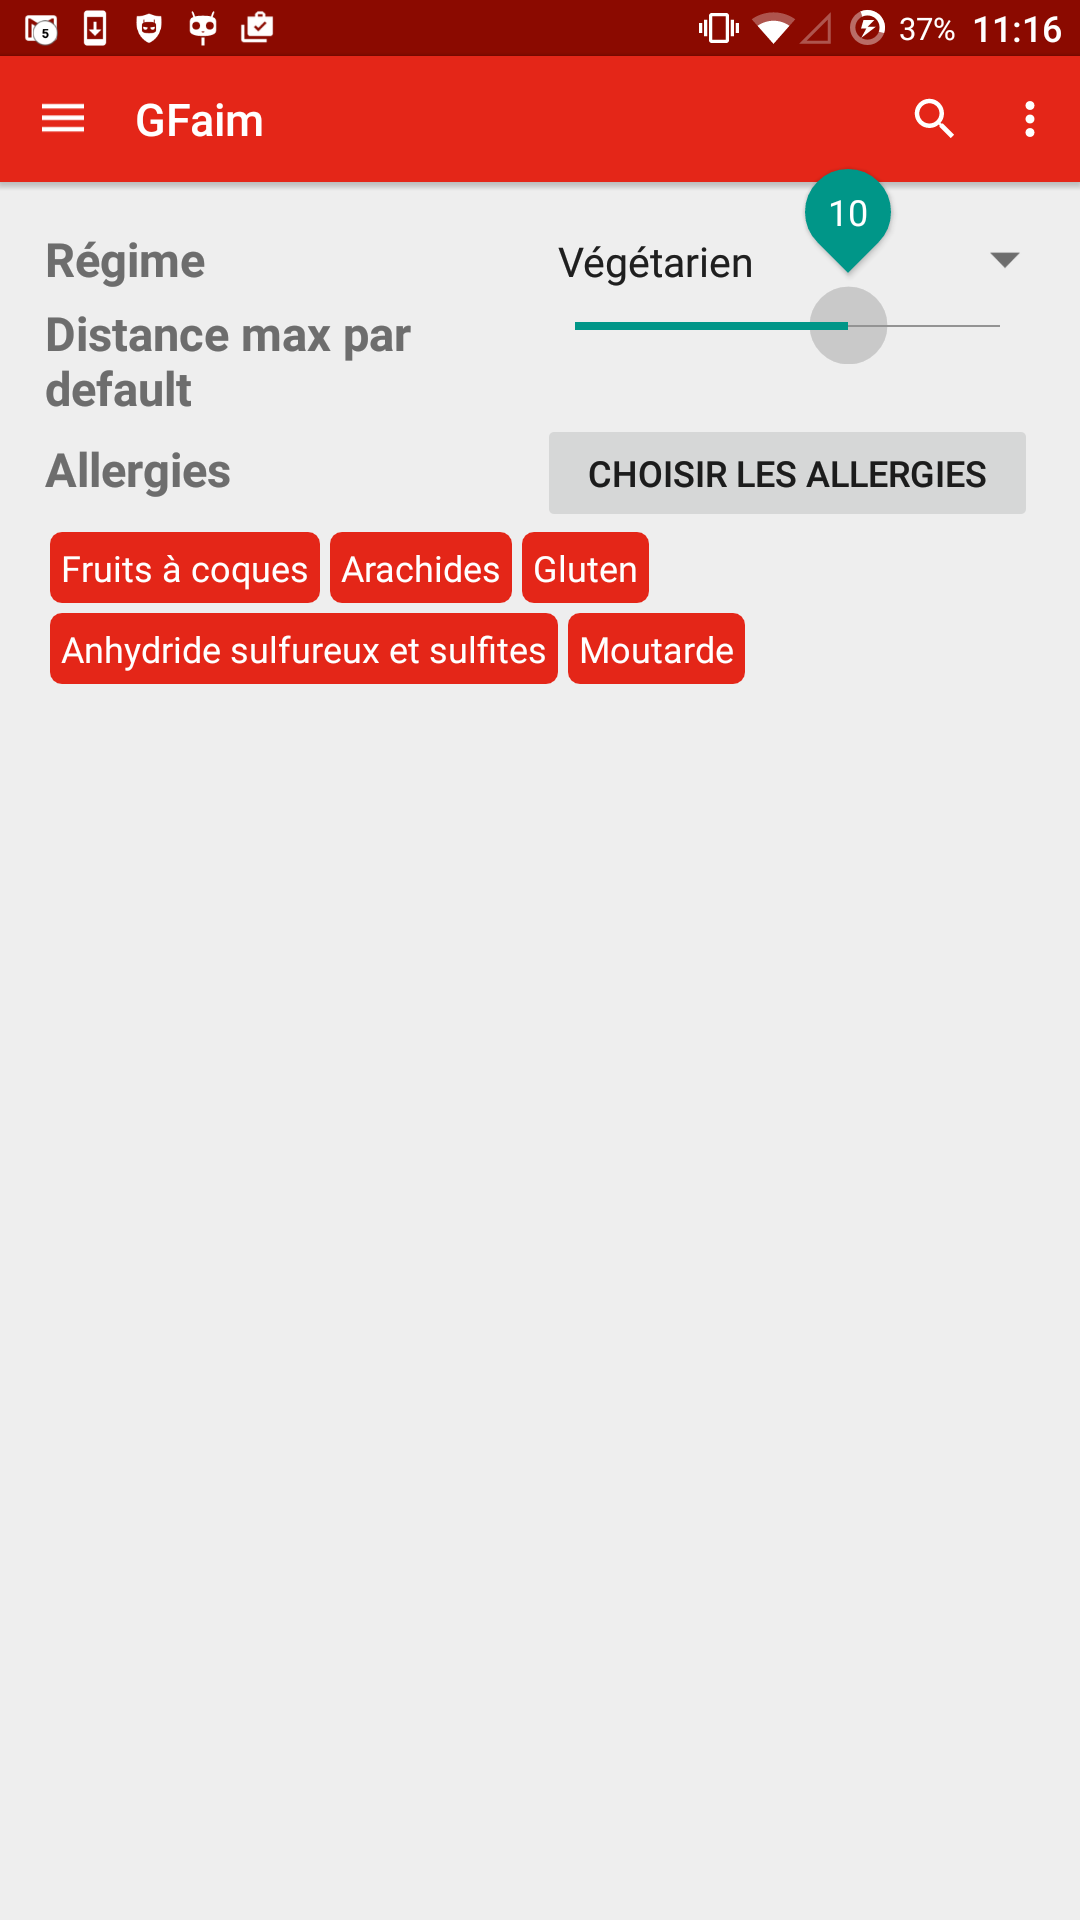
\includegraphics[width=8cm]{figures/screenshots/screenshot_preferences.png}}
    \caption{Capture d'écran de configuration des préférences}
\end{figure}

\begin{figure}[H]
    \label{fig-recherche-avancee}
    \noindent\makebox[\textwidth]{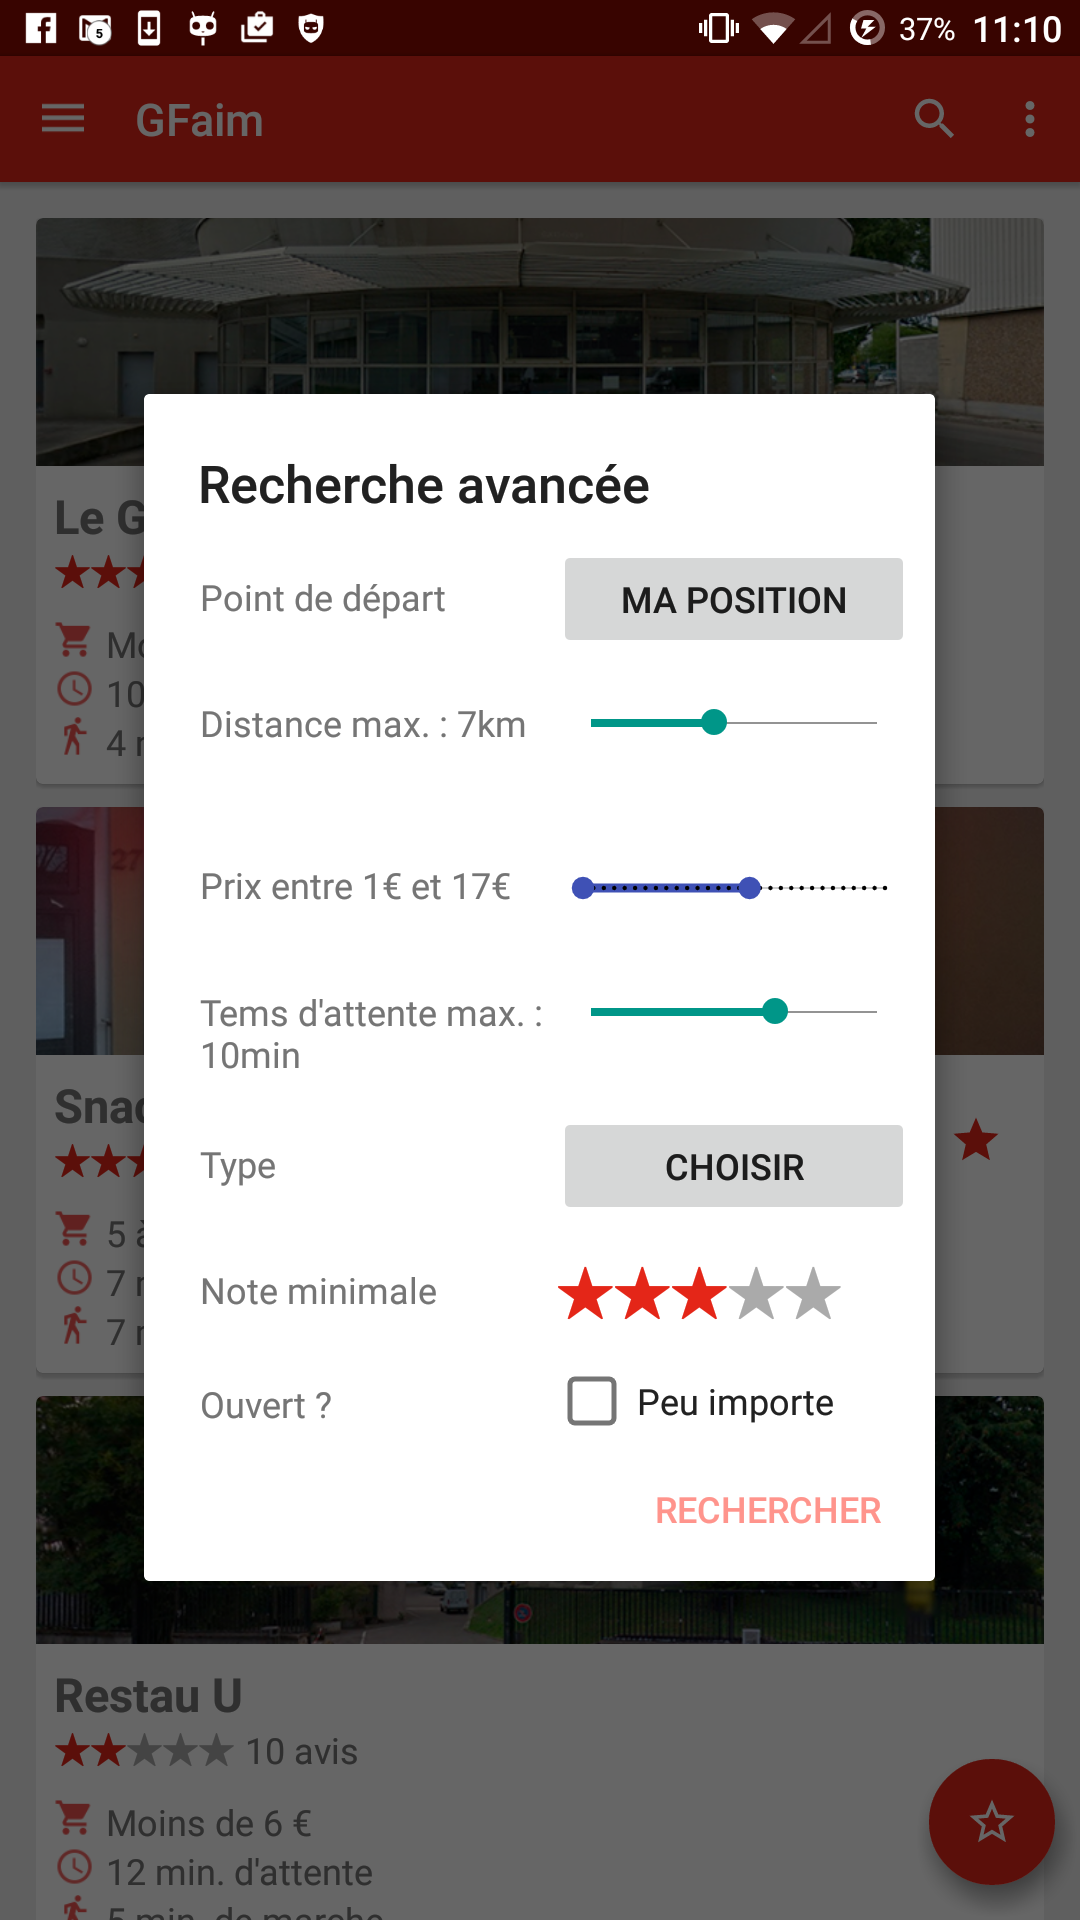
\includegraphics[width=8cm]{figures/screenshots/screenshot_recherche_avancee.png}}
    \caption{Capture d'écran de la recherche avancée}
\end{figure}

\begin{figure}[H]
    \label{fig-reglage-alarme}
    \noindent\makebox[\textwidth]{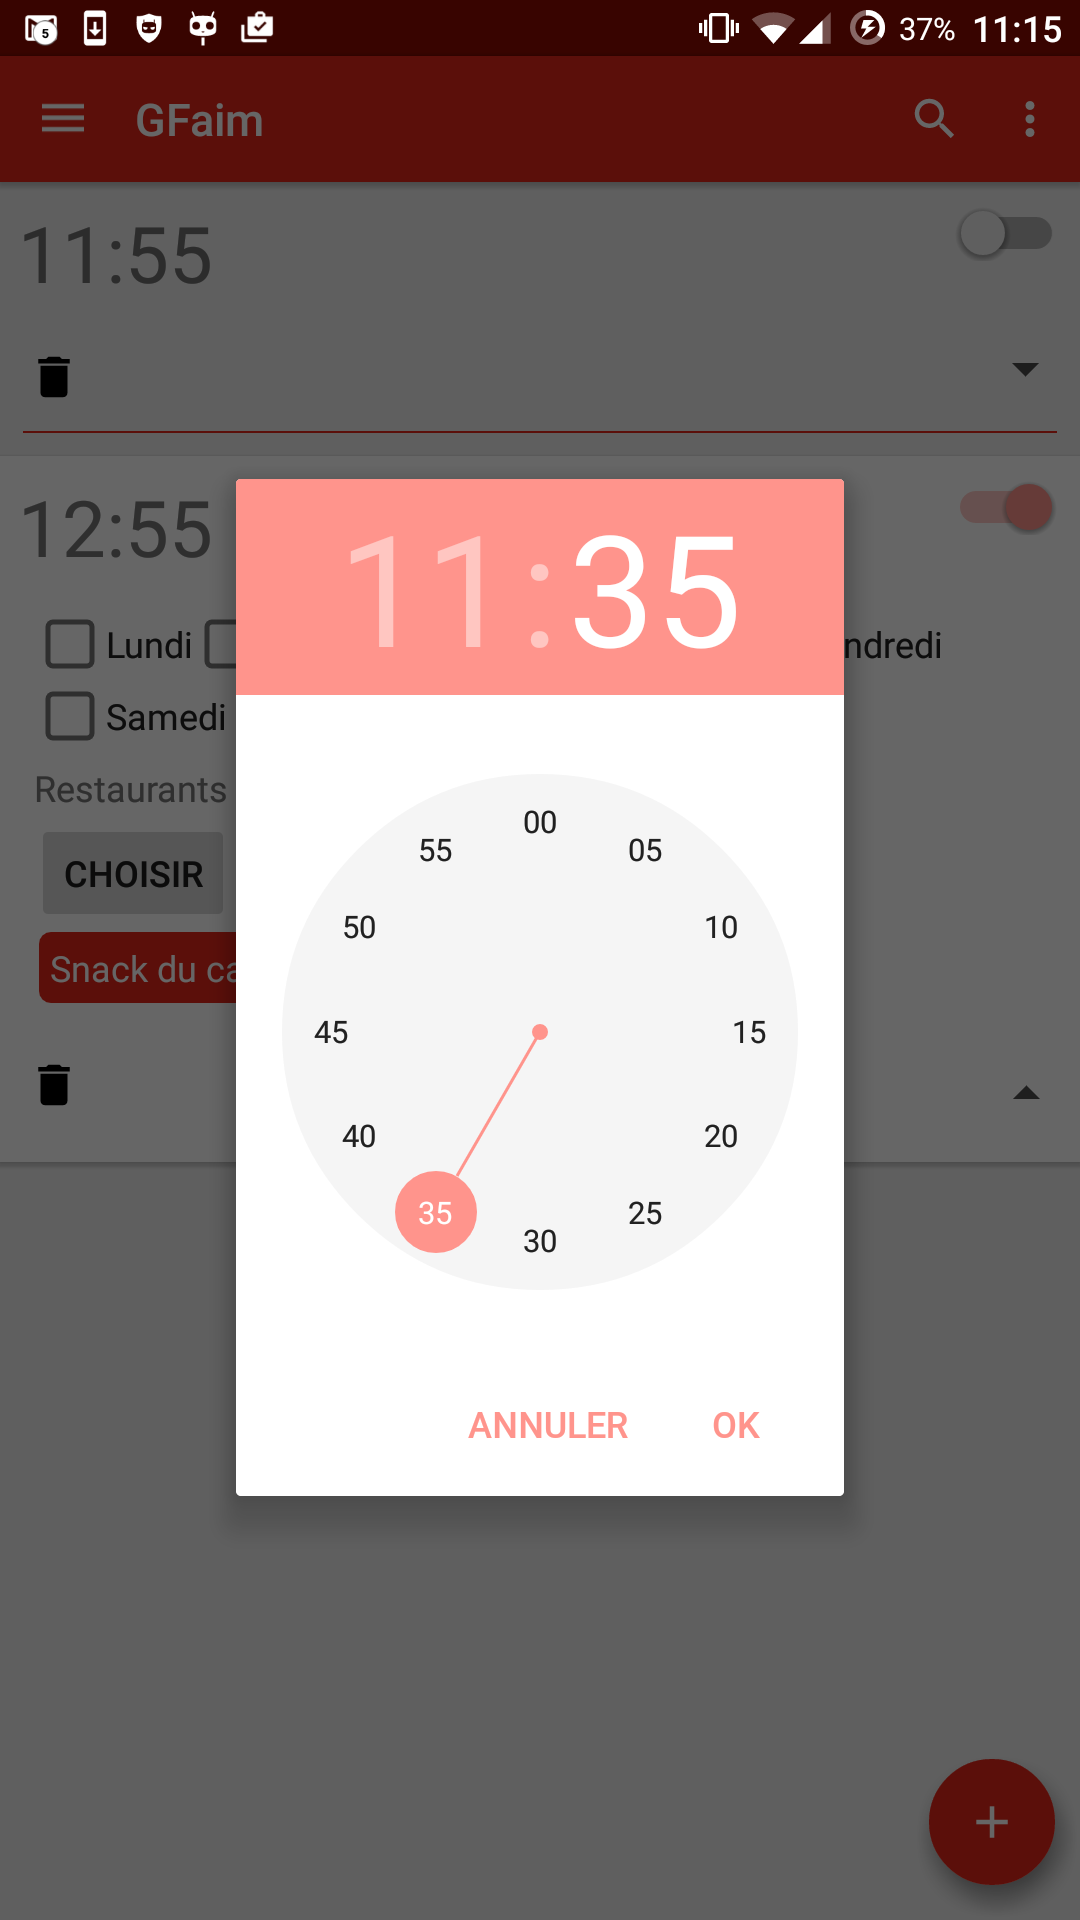
\includegraphics[width=8cm]{figures/screenshots/screenshot_reglage_alarme.png}}
    \caption{Capture d'écran du réglage de l'alarme}
\end{figure}

\begin{figure}[H]
    \label{fig-zoom-photo}
    \noindent\makebox[\textwidth]{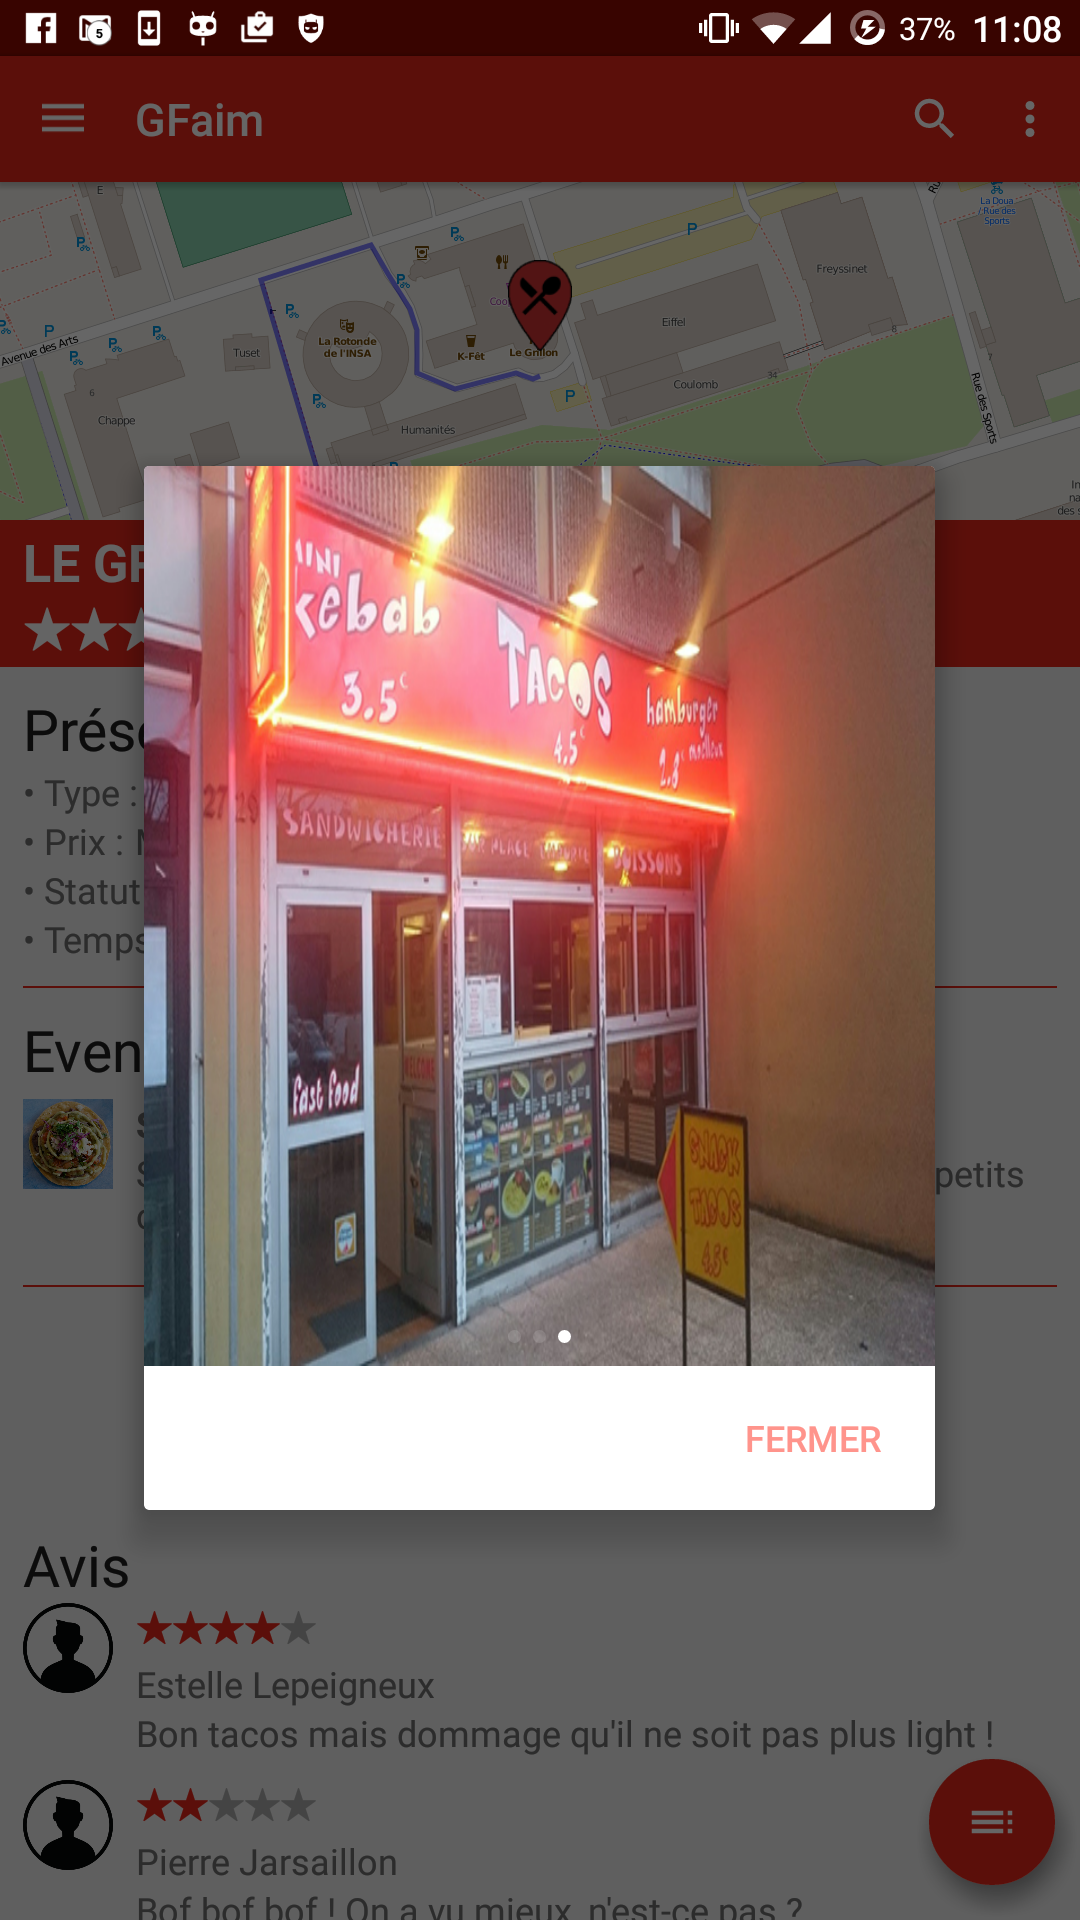
\includegraphics[width=8cm]{figures/screenshots/screenshot_zoom_photo_restaurant.png}}
    \caption{Capture d'écran de la vue zoom photo}
\end{figure}


\subsection{Guide pour le consommateur}

Que vous soyez restaurateur ou simple consommateur, les fonctionnalités décrite dans la suite peuvent vous intéresser. \\

\begin{description}
    \item \bf{Consulter les restaurants :} \\ \\
        Pour consulter la liste des restaurants situés aux alentours, il faut d'abord ouvrir le volet déroulant sur la gauche. Pour ce faire, il existe deux manières de procéder (la première n'étant possible que sur certaines fenêtres de l’application) : soit en appuyant sur le bouton d'ouverture du menu en haut à gauche (trois petites barres horizontales), soit en faisant glisser votre doigt de la gauche vers la droite sur votre écran. \\
        Ensuite, il y a deux façons de procéder : pour la première, cliquez sur l'onglet \og{}Restaurants\fg{} pour voir la liste des restaurants proches, vos restaurants favoris étant mis en avant s'ils sont dans les environs. Une vue succinte de plusieurs restaurants s'affiche alors, avec le nom du restaurant, l'avis moyen des utilisateurs, une distance par rapport à vous, éventuellement une photo\dots~La deuxième façon de voir des restaurants est d'utiliser la carte. Cliquez alors sur l’onglet \og{}Carte\fg{}. Vous accéderez alors à la vue d'une cartographie, qui sera par défaut centrée sur votre position et qui vous indiquera, grâce à des marqueurs de position, les restaurants situés dans les environs. En cliquant sur l'un des marqueurs, une petite info-bulle contenant les mêmes informations que celles citées précédemment s’affichera. \\

    \item \bf{Consulter les détails d'un restaurants :} \\ \\
        Pour consulter le détail d'un restaurant, il faut d'abord obtenir une liste de restaurants, soit en passant par la recherche (voir cas suivants), soit en utilisant l'onglet \og{}Restaurants\fg{} du volet déroulant (voir cas précédent). Cliquez sur l'un des restaurants de la liste pour consulter son détail. Vous arriverez sur une page recensant nombre d'informations utiles sur le restaurant, comme le temps d’attente pour avoir votre plat, les avis détaillés des utilisateurs, la distance par rapport à votre position actuelle, le type de restaurant, les prix pratiqués, les horaires du restaurant\dots~Mais également les événements à venir, les commodités dont dispose le restaurant (wifi gratuit, à emporter, terrasse\dots) ou encore une carte permettant de situer le restaurant. \\
        En dessous de la carte, vous pourrez constater la présence de six icônes : \\
            \begin{description}
                \item[\textbullet] La première permet d’accéder aux photos du restaurant. 
                \item[\textbullet] La deuxième permet d’afficher le numéro de téléphone du restaurant.
                \item[\textbullet] La troisième vous renvoie vers son site web. 
                \item[\textbullet] La quatrième vous offre la possibilité de laisser une note et un avis. 
                \item[\textbullet] La cinquième permet d’ajouter le restaurant à vos favoris. 
                \item[\textbullet] Et enfin, la dernière vous amène au menu du restaurant. \\
            \end{description}

    \item \bf{Rechercher un restaurant en particulier :} \\ \\
        En haut à droite des fenêtres principales de l'application (carte, liste des restaurants, réglages des alarmes), une petite loupe est affichée. Cliquez dessus pour faire apparaître la barre de rechercher. Entrez le nom du restaurant que vous recherchez. Une liste de restaurants correspondant aux mots entrés s'affichera alors dynamiquement au fur et à mesure que vous écrivez. Si vous avez entré un nom précis et unique, un seul restaurant sera affiché dans la liste. Si le nom recherché est plus générique, vous devrez trouver votre restaurant parmi ceux affichés dans la liste. \\
        
    \item \bf{Rechechercher des restaurants :} \\ \\
        Pour rechercher des restaurants sur critères particuliers (prix, distance, etc.), utilisez la recherche avancée. Pour ce faire, cliquez sur la loupe située en haut à droite de l'écran des fenêtres principales et cliquez ensuite sur \og{}Recherche avancée\fg{}. Une nouvelle fenêtre s'ouvrira alors, vous offrant un panel de critères à régler, comme le temps d'attente du restaurant, la note moyenne minimale des utilisateurs, s'il dispose du wifi gratuit, s'il est ouvert actuellement\dots~Cliquez ensuite sur \og{}Ok\fg{} pour lancer la recherche. Une liste de restaurants correspondant aux critères indiqués apparaîtra alors. \\
        
    \item \bf{Paramétrer une alarme :} \\ \\
        Afin de paramétrer une alarme, il faut d'abord accéder à la fenêtre \og{}Alarmes\fg{}. Ouvrez alors le volet déroulant sur la gauche comme expliqué dans le cas \og{}Consuler des restaurants\fg{}. Cliquez ensuite sur \og{}Alarmes\fg{}. Vous arrivez sur une fenêtre où vous pouvez consulter la liste des alarmes que vous avez déjà programmées, et les activer désactiver en cliquant sur le switch en haut à droite de chaque alarme, ou bien voir leur détail en cliquant sur le bouton \og{}triangle inversé\fg{} en bas à droite de chaque alarme. Vous pourrez alors modifier les jours par défaut, les restaurants concernés par l'alarme, ou encore supprimer complètement l'alarme. En cliquant sur le bouton \og{}Ajouter\fg{}, vous pourrez créer une nouvelle alarme en paramétrant tous les détails indiqués ci-dessus.
        
\end{description}

\subsection{Guide pour le restaurateur}

Vous trouverez ci dessous les différentes fonctionnalités propres à votre rôle de restaurateur. N'oubliez pas de lire la section précédente qui vous concerne aussi en tant que consommateur. \\

\begin{description}
    \item \bf{Modifier les informations générales concernant mon restaurant :} \\ \\
    Afin de modifier les infos générales de votre restaurant, il faut tout d'abord accéder à la liste de votre restaurant (liste ne contenant qu'un restaurant si vous n'en possédez qu'un). Pour ce faire, il faut d'abord ouvrir le volet déroulant sur la gauche. Il existe deux manières de procéder (la première n'étant possible que sur certaines fenêtres de l’application) : soit en appuyant sur le bouton d'ouverture du menu en haut à gauche (trois petites barres horizontales), soit en faisant glisser votre doigt de la gauche vers la droite sur votre écran. Cliquer ensuite sur l’onglet \og{}Mes Restaurants\fg{}, puis sélectionner le restaurant dont vous voulez modifier les informations. Vous arriverez alors par défaut sur l'onglet recensant les informations principales. Vous pouvez les modifier directement dans les champs prévus à cet effet puis valider les modifications en cliquant sur le bouton \og{}Valider\fg{}. \\

    \item \bf{Changer le menu de mon restaurant :} \\ \\
    Pour changer le menu de votre restaurant, le début de la démarche est le même que pour modifier les informations générales : ouvrez le volet déroulant sur la gauche, sélectionnez \og{}Mes restaurants\fg{}, puis le restaurant dont vous souhaitez changer le menu. Par défaut, vous arrivez sur l'onglet \og{}Informations générales\fg{}. Cliquez alors sur l'onglet \og{}Menu\fg{} (deuxième onglet en bas). Vous pourrez alors modifier votre menu soit en envoyant un scan ou des photos de votre menu, soit en le tapant directement sur le clavier de votre téléphone. \\
        
    \item \bf{Ajouter des photos de mon restaurant :} \\ \\
    Pour ajouter des photos de votre restaurant, le début de la démarche est le même que pour modifier les informations générales : ouvrez le volet déroulant sur la gauche, sélectionnez \og{}Mes restaurants\fg{}, puis le restaurant pour lequel vous souhaitez ajouter des photos. Par défaut, vous arrivez sur l'onglet \og{}Informations générales\fg{}. Cliquez alors sur l’onglet \og{}Ajouter photos\fg{} (troisième onglet en bas). Vous pourrez alors ajouter des photos de votre restaurant pour lui apporter plus de visiblité et de crédibilité auprès des utilisateurs de l'application. \\

    \item \bf{Ajouter un événement pour mon restaurant :} \\ \\
    Pour ajouter un événement pour votre restaurant, le début de la démarche est le même que pour modifier les informations générales : ouvrez le volet déroulant sur la gauche, sélectionnez \og{}Mes restaurants\fg{}, puis le restaurant pour lequel vous souhaitez ajouter un événement. Par défaut, vous arrivez sur l'onglet \og{}Informations générales\fg{}. Cliquez alors sur l'onglet \og{}Ajouter événement\fg{} (quatrième onglet en bas). Vous pourrez alors ajouter un événement pour votre restaurant (soirée dansante, invités spéciaux, promotions sur un menu\dots) en remplissant les champs nécessaires. \\
    
\end{description}